%%%%%%%%%%%%%%%%%%%%%%%%%%%%%%%%%%%%%%%%%%%%%%%%%%%
\begin{frame}
  \begin{center}
    {\Large Introduction to PyTorch}
    
\tiny{(Ref: Pytorch Official documentation + few other sources, like Lyman Lin (NTU)))}
  \end{center}
\end{frame}

%%%%%%%%%%%%%%%%%%%%%%%%%%%%%%%%%%%%%%%%%%%%%%%%%%%
\begin{frame}[fragile] \frametitle{What is PyTorch?}
  \begin{center}

{\Large Pytorch is a Python-based scientific computing package that is a replacement for NumPy, and uses the power of Graphics Processing Units. It is also a deep learning research platform that provides maximum flexibility and speed.}

  \end{center}

  {\tiny (Ref: How Pytorch gives the big picture with deep learning - Déborah Mesquita)}
\end{frame}

%%%%%%%%%%%%%%%%%%%%%%%%%%%%%%%%%%%%%%%%%%%%%%%%%%%
\begin{frame}[fragile] \frametitle{What is PyTorch?}
\begin{itemize}
\item  Developed by Facebook
\item torch in Lua but Pytorch in python fully
\item Similar to numpy but leverages GPU
\item Deep Learning Library
\item  Dynamic Neural Network
\end{itemize}
\begin{center}

\includegraphics[width=0.8\linewidth,keepaspectratio]{pyt4}
\end{center}
\end{frame}

%%%%%%%%%%%%%%%%%%%%%%%%%%%%%%%%%%%%%%%%%%%%%%%%%%%
\begin{frame}[fragile] \frametitle{Installation}

\begin{itemize}
\item  http://pytorch.org/ for Linux and Mac
\begin{center}
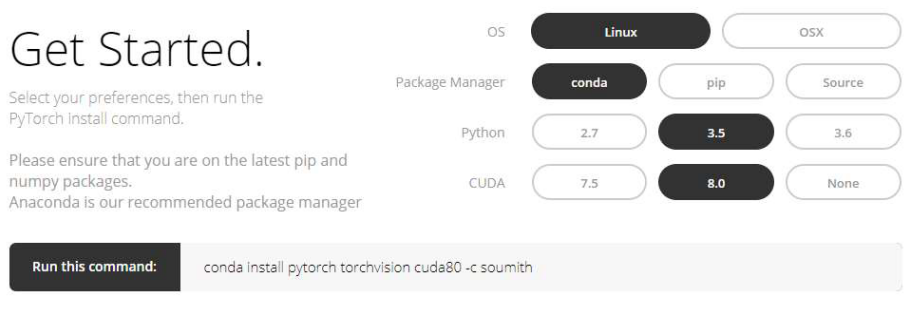
\includegraphics[width=\linewidth,keepaspectratio]{pyt5}
\end{center}
\item For windows \lstinline|conda install -c peterjc123 pytorch|
\end{itemize}

\end{frame}


%%%%%%%%%%%%%%%%%%%%%%%%%%%%%%%%%%%%%%%%%%%%%%%%%%%
\begin{frame}[fragile] \frametitle{Imp Packages inside PyTorch}
\begin{itemize}
\item  torch: a Tensor library like Numpy, with strong GPU support
\item torch.autograd: an automatic differentiation library 
\item torch.nn: a neural networks library deeply integrated with autograd 
\item torch.optim: an optimization package to be used with torch.nn
\item torch.utils: DataLoader, Trainer and other utility functions for convenience
\end{itemize}
\end{frame}


%%%%%%%%%%%%%%%%%%%%%%%%%%%%%%%%%%%%%%%%%%%%%%%%%%%
\begin{frame}[fragile] \frametitle{Concepts of PyTorch}
\begin{itemize}
\item Data:
\begin{itemize}
\item  Tensor
\item Variable (for Gradient)
\end{itemize}
\item Function:
\begin{itemize}
\item   NN Modules
\item   Optimizer
\item   Loss Function
\item   Multi-Processing
\end{itemize}
\end{itemize}
\end{frame}




%%%%%%%%%%%%%%%%%%%%%%%%%%%%%%%%%%%%%%%%%%%%%%%%%%%
\begin{frame}[fragile] \frametitle{Fundamental Data Types}
Tensors: Similar to numpy ndarry but leverage GPU
\begin{lstlisting}
import torch

x = torch.Tensor(5, 3)
print(x)

0.0000   0.0000   0.0001
  0.0000   0.0001   0.0000
  3.3717   0.0000   3.3717
  0.0000   3.8859   0.0000
  3.8001   0.0000  27.0173
[torch.FloatTensor of size 5x3]
\end{lstlisting}
\end{frame}

%%%%%%%%%%%%%%%%%%%%%%%%%%%%%%%%%%%%%%%%%%%%%%%%%%%
\begin{frame}[fragile] \frametitle{Fundamental Data Types}
Construct a randomly initialized matrix
\begin{lstlisting}
import torch

x = torch.rand(5, 3)
print(x)

0.5357  0.7362  0.2274
 0.5483  0.0888  0.9738
 0.9148  0.4890  0.3909
 0.5597  0.3481  0.9360
 0.5883  0.8458  0.1757
[torch.FloatTensor of size 5x3]
\end{lstlisting}
\end{frame}


%%%%%%%%%%%%%%%%%%%%%%%%%%%%%%%%%%%%%%%%%%%%%%%%%%%
\begin{frame}[fragile] \frametitle{DataLoaders}
Simple data-loader, manual, and feeding ALL data to the model. No batch!!
\begin{lstlisting}
xy = np.loadtxt('./data/diabetes.csv', delimiter=',', dtype=np.float32)
x_data = Variable(torch.from_numpy(xy[:, 0:-1]))
y_data = Variable(torch.from_numpy(xy[:, [-1]]))

# Training loop
for epoch in range(100):
        # Forward pass: Compute predicted y by passing x to the model
    y_pred = model(x_data)

    # Compute and print loss
    loss = criterion(y_pred, y_data)
    print(epoch, loss.data[0])

    # Zero gradients, perform a backward pass, and update the weights.
    optimizer.zero_grad()
    loss.backward()
    optimizer.step()
\end{lstlisting}

\tiny{(Ref: PyTorchZeroToAll  - Sung Kim)}
\end{frame}

%%%%%%%%%%%%%%%%%%%%%%%%%%%%%%%%%%%%%%%%%%%%%%%%%%%
\begin{frame}[fragile] \frametitle{DataLoaders}
\begin{itemize}
\item For big-data, we can not feed ALL. 
\item Need to divide into batches. 
\item Feed one batch at a time. 
\item Compute gradients.
\item Update weights.
\item \textbf{epoch}: One forward pass and one backward pass for ALL training rows.
\item \textbf{batch\_size}: Number of training rows in one forward/backward pass.
\item \textbf{iterations}: Number of passes in one epoch. One batch iteration. Training rows divided by batch\_size
\end{itemize}
\begin{lstlisting}
# Training loop
for epoch in range(100):
   for i in range(total_batches):
   	batch_xs, batch_ys = ...
\end{lstlisting}

\tiny{(Ref: PyTorchZeroToAll  - Sung Kim)}
\end{frame}

%%%%%%%%%%%%%%%%%%%%%%%%%%%%%%%%%%%%%%%%%%%%%%%%%%%
\begin{frame}[fragile] \frametitle{DataLoaders}
Data loader takes care of batching and scuffling and gives out iterable for batches.
\begin{center}
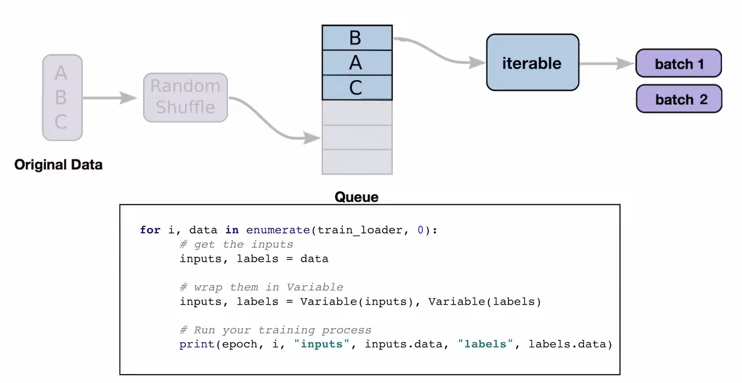
\includegraphics[width=0.8\linewidth,keepaspectratio]{pyhun28}
\end{center}

\tiny{(Ref: PyTorchZeroToAll  - Sung Kim)}
\end{frame}

%%%%%%%%%%%%%%%%%%%%%%%%%%%%%%%%%%%%%%%%%%%%%%%%%%%
\begin{frame}[fragile] \frametitle{DataLoaders}
For our own dataset, create own dataloader.
\begin{center}
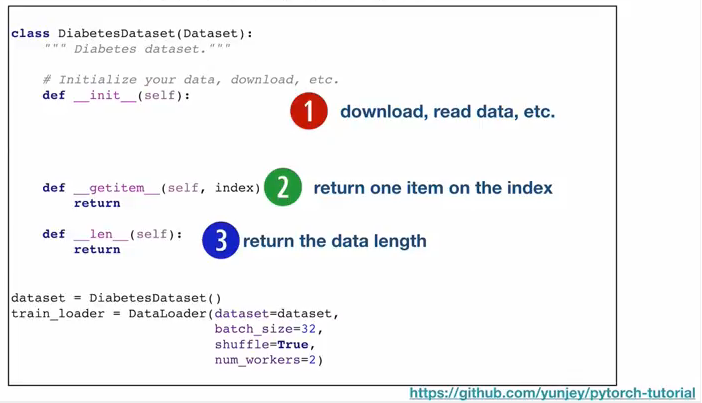
\includegraphics[width=0.8\linewidth,keepaspectratio]{pyhun29}
\end{center}

\tiny{(Ref: PyTorchZeroToAll  - Sung Kim)}
\end{frame}

%%%%%%%%%%%%%%%%%%%%%%%%%%%%%%%%%%%%%%%%%%%%%%%%%%%
\begin{frame}[fragile] \frametitle{DataLoaders}
For diabetics csv, here is the dataloader
\begin{center}
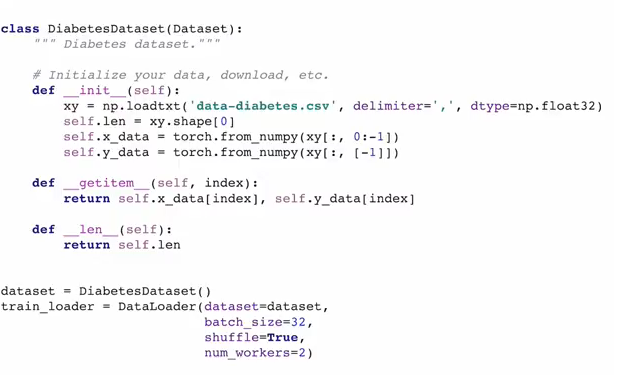
\includegraphics[width=0.8\linewidth,keepaspectratio]{pyhun30}
\end{center}

\tiny{(Ref: PyTorchZeroToAll  - Sung Kim)}
\end{frame}


%%%%%%%%%%%%%%%%%%%%%%%%%%%%%%%%%%%%%%%%%%%%%%%%%%%
\begin{frame}[fragile] \frametitle{DataLoaders}
Some famous datasets are in pytorch itself.
\begin{center}
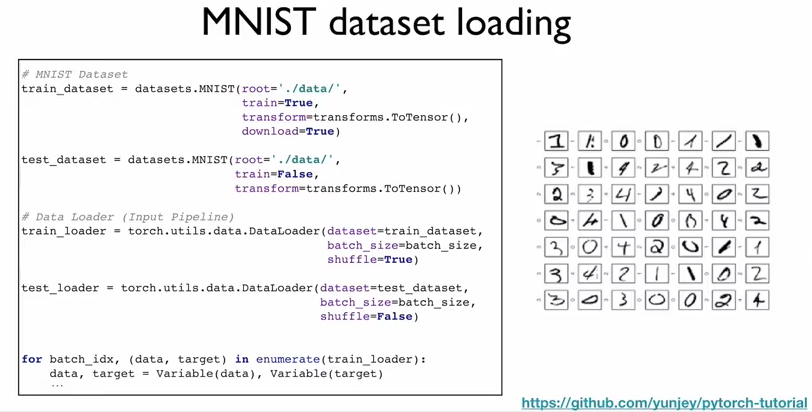
\includegraphics[width=0.8\linewidth,keepaspectratio]{pyhun31}
\end{center}

\tiny{(Ref: PyTorchZeroToAll  - Sung Kim)}
\end{frame}


%%%%%%%%%%%%%%%%%%%%%%%%%%%%%%%%%%%%%%%%%%%%%%%%%%%
\begin{frame}[fragile] \frametitle{Operations}
Additions
\begin{lstlisting}
x = torch.Tensor(5, 3)
y = torch.rand(5, 3)
print(x + y)

print(torch.add(x, y))

result = torch.Tensor(5, 3)
torch.add(x, y, out=result)

y.add_(x)
\end{lstlisting}
\end{frame}

%%%%%%%%%%%%%%%%%%%%%%%%%%%%%%%%%%%%%%%%%%%%%%%%%%%
\begin{frame}[fragile] \frametitle{Numpy Bridge}
\begin{itemize}
\item Converting a torch Tensor to a numpy array and vice versa. 
\item The torch Tensor and numpy array will share their underlying memory locations, and changing one will change the other.
\end{itemize}

\begin{lstlisting}
a = torch.ones(5)
b = a.numpy()
a.add_(1)

print(a)
print(b)
# both are with same values
\end{lstlisting}
\end{frame}

%%%%%%%%%%%%%%%%%%%%%%%%%%%%%%%%%%%%%%%%%%%%%%%%%%%
\begin{frame}[fragile] \frametitle{Numpy Bridge}
Converting numpy Array to torch Tensor

\begin{lstlisting}
import numpy as np
a = np.ones(5)
b = torch.from_numpy(a)
np.add(a, 1, out=a)
print(a)
print(b)

[ 2.  2.  2.  2.  2.]

 2
 2
 2
 2
 2
[torch.DoubleTensor of size 5]
\end{lstlisting}
All the Tensors on the CPU except a CharTensor support converting to NumPy and back.
\end{frame}

%%%%%%%%%%%%%%%%%%%%%%%%%%%%%%%%%%%%%%%%%%%%%%%%%%%
\begin{frame}[fragile] \frametitle{CUDA Tensors}
Tensors can be moved onto GPU using the .cuda function.

\begin{lstlisting}
# let us run this cell only if CUDA is available
if torch.cuda.is_available():
    x = x.cuda()
    y = y.cuda()
    x + y

\end{lstlisting}
\end{frame}

%%%%%%%%%%%%%%%%%%%%%%%%%%%%%%%%%%%%%%%%%%%%%%%%%%%
\begin{frame}[fragile] \frametitle{Autograd: automatic gradient}
\begin{itemize}
\item Provides automatic differentiation for all operations on Tensors
\item It is a define-by-run framework, which means that your backprop is defined by how your code is run, and that every single iteration can be different.
\end{itemize}
\end{frame}

%%%%%%%%%%%%%%%%%%%%%%%%%%%%%%%%%%%%%%%%%%%%%%%%%%%
\begin{frame}[fragile] \frametitle{Dynamic Computation Graphs}

\begin{center}
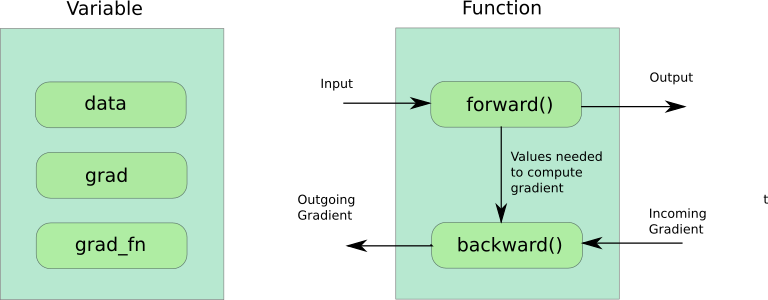
\includegraphics[width=\linewidth,keepaspectratio]{pyt38}
\end{center}
PyTorch 0.4 merges the Variable and Tensor class into one, and Tensor can be made into a “Variable” by a switch rather than instantiating a new object. 

{\tiny (Ref: Getting Started with PyTorch Part 1: Understanding how Automatic Differentiation works - Ayoosh Kathuria )}
\end{frame}


%%%%%%%%%%%%%%%%%%%%%%%%%%%%%%%%%%%%%%%%%%%%%%%%%%%
\begin{frame}[fragile] \frametitle{Variable}
\begin{itemize}
\item autograd.Variable wraps a Tensor, and supports nearly all of operations defined on it.
\item Records the history of operations applied to it. 
\item Has the same API as a Tensor, with some additions like backward(). 
\item Also holds the gradient w.r.t. the tensor.
\item call .backward() and have all the gradients computed automatically.
\end{itemize}
\begin{center}
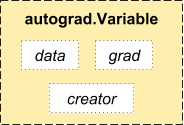
\includegraphics[width=0.4\linewidth,keepaspectratio]{pyt1}
\end{center}
\end{frame}

%%%%%%%%%%%%%%%%%%%%%%%%%%%%%%%%%%%%%%%%%%%%%%%%%%%
\begin{frame}[fragile] \frametitle{Function}
\begin{itemize}
\item Implements forward and backward definitions of an autograd operation. 
\item Every Variable operation, creates at least a single Function node, that connects to functions that created a Variable and encodes its history.
\item Variable and Function are interconnected and build up an acyclic graph, that encodes a complete history of computation.
\item Each variable has a .grad\_fn attribute that references a Function that has created the Variable (except for Variables created by the user - their grad\_fn is None).
\end{itemize}
\end{frame}



%%%%%%%%%%%%%%%%%%%%%%%%%%%%%%%%%%%%%%%%%%%%%%%%%%%
\begin{frame}[fragile] \frametitle{Define the network}
 With TensorFlow each layer operation has to be explicitly named:

 \begin{lstlisting}
def multilayer_perceptron(input_tensor, weights, biases):
    layer_1_multiplication = tf.matmul(input_tensor, weights['h1'])
    layer_1_addition = tf.add(layer_1_multiplication, biases['b1'])
    layer_1_activation = tf.nn.relu(layer_1_addition)
    
    layer_2_multiplication = tf.matmul(layer_1_activation, weights['h2'])
    layer_2_addition = tf.add(layer_2_multiplication, biases['b2'])
    layer_2_activation = tf.nn.relu(layer_2_addition)
    
    out_layer_multiplication = tf.matmul(layer_2_activation, weights['out'])
    out_layer_addition = out_layer_multiplication + biases['out']
    
    return out_layer_additio
\end{lstlisting}

  {\tiny (Ref: How Pytorch gives the big picture with deep learning - Déborah Mesquita)}
\end{frame}

%%%%%%%%%%%%%%%%%%%%%%%%%%%%%%%%%%%%%%%%%%%%%%%%%%%
\begin{frame}[fragile] \frametitle{Define the network}
\begin{itemize}
\item With Pytorch we use torch.nn. 
\item We need to multiply each input node with a weight, and also to add a bias. 
\item The class torch.nn.Linear does the job for us.
\item The base class for all neural network modules is torch.nn.Module.
\item The forward(*input) defines the computation performed at every call, and all subclasses should override it.
\item forward() takes inputs, takes it through all the layers and returns the output. Almost like predict the output, with current weights.
\end{itemize}

  {\tiny (Ref: How Pytorch gives the big picture with deep learning - Déborah Mesquita)}
\end{frame}


%%%%%%%%%%%%%%%%%%%%%%%%%%%%%%%%%%%%%%%%%%%%%%%%%%%
\begin{frame}[fragile] \frametitle{Define the network}
 \begin{lstlisting}
class OurNet(nn.Module):
 def __init__(self, input_size, hidden_size, num_classes):
     super(Net, self).__init__()
     self.layer_1 = nn.Linear(n_inputs,hidden_size, bias=True)
     self.relu = nn.ReLU()
     self.layer_2 = nn.Linear(hidden_size, hidden_size, bias=True)
     self.output_layer = nn.Linear(hidden_size, num_classes, bias=True)
 
 def forward(self, x):
     out = self.layer_1(x)
     out = self.relu(out)
     out = self.layer_2(out)
     out = self.relu(out)
     out = self.output_layer(out)
     return out
\end{lstlisting}

  {\tiny (Ref: How Pytorch gives the big picture with deep learning - Déborah Mesquita)}
\end{frame}

%%%%%%%%%%%%%%%%%%%%%%%%%%%%%%%%%%%%%%%%%%%%%%%%%%%
\begin{frame}[fragile] \frametitle{Define the network}
\begin{itemize}
\item In \_\_init\_\_ we need to call super class's constructor and define the layers. This gets called when we say $model = MyModel()$
\item forward() is the call that takes the input and dynamically constructs the graph. This gets called when we call $model(x)$ inside the epoch loop. So, this forward call gets called in each iteration, creating dynamic graph each time.
\item With this, depending on the size of input, we can dynamically construct NN accordingly, useful for variable length sequences.
\end{itemize}

\end{frame}


%%%%%%%%%%%%%%%%%%%%%%%%%%%%%%%%%%%%%%%%%%%%%%%%%%%
\begin{frame}[fragile] \frametitle{Update the weights}
\begin{itemize}
\item The way the neural network ''learns'' is by updating the weight values. With Pytorch we use the torch.autograd package to do that.
\item We didn’t specify the weight tensors like we did with TensorFlow because the torch.nn.Linear class has a variable weight with shape (out\_features x in\_features).
\item torch.nn.Linear(in\_features, out\_features, bias=True)
\end{itemize}

  {\tiny (Ref: How Pytorch gives the big picture with deep learning - Déborah Mesquita)}
\end{frame}

%%%%%%%%%%%%%%%%%%%%%%%%%%%%%%%%%%%%%%%%%%%%%%%%%%%
\begin{frame}[fragile] \frametitle{Update the weights}
\begin{itemize}
\item To compute the gradient, we will use the the method Adaptive Moment Estimation (Adam). Torch.optim is a package that implements various optimization algorithms.
\item To use torch.optim, you have to construct an optimizer object that will hold the current state and also update the parameters based on the computed gradients.
\item To construct an optimizer, you have to give it an iterable that contains the parameters (all should be variables ) to optimize. Then you can specify options that are specific to an optimizer, such as the learning rate, weight decay, etc.
\end{itemize}


  {\tiny (Ref: How Pytorch gives the big picture with deep learning - Déborah Mesquita)}
\end{frame}

%%%%%%%%%%%%%%%%%%%%%%%%%%%%%%%%%%%%%%%%%%%%%%%%%%%
\begin{frame}[fragile] \frametitle{Update the weights}
Typical Optimization workflow

 \begin{lstlisting}
for input, target in dataset:
	optimizer.zero_grad()
	output = model(input) # calls model.forward()
	loss = loss_fn(output, target)
	loss.backward()
	optimizer.step()
\end{lstlisting}

As ``loss'' is formulated in terms of ``output'' which is in terms of inputs and weights, when we say loss.backward(), autograd does backprop and sets gradient values in all input variables. Gradients are evaluated at the predicted output (not target given)

optimizer.step() updates the weights (also called Parameters). Once weights are updated, the gradient values stored in input variables are useless. They are set to zero before next network is back-propagated. Its done by optimizer.zero\_grad()

  {\tiny (Ref: PyTorch: Fast Differentiable Dynamic Graphs in Python - Soumith Chintala)}
\end{frame}


%%%%%%%%%%%%%%%%%%%%%%%%%%%%%%%%%%%%%%%%%%%%%%%%%%%
\begin{frame}[fragile] \frametitle{Update the weights}


 \begin{lstlisting}
net = OurNet(input_size, hidden_size, num_classes)
criterion = nn.CrossEntropyLoss()
optimizer = torch.optim.Adam(net.parameters(), lr=learning_rate)
for t in range(500):
    y_pred = net(x)
    loss = criterion(y_pred, y)
    optimizer.zero_grad()
    loss.backward()
    optimizer.step()
\end{lstlisting}

  {\tiny (Ref: How Pytorch gives the big picture with deep learning - Déborah Mesquita)}
\end{frame}


%%%%%%%%%%%%%%%%%%%%%%%%%%%%%%%%%%%%%%%%%%%%%%%%%%%
\begin{frame}[fragile] \frametitle{Update the weights}
\begin{itemize}
\item To compute the loss we'll use torch.nn.CrossEntropyLoss
\item 
One important thing about torch.nn.CrossEntropyLoss is that input has to be a 2D tensor of size (minibatch, n) and target expects a class index (0 to nClasses-1) as the target for each value of a 1D tensor of size minibatch.
\end{itemize}

  {\tiny (Ref: How Pytorch gives the big picture with deep learning - Déborah Mesquita)}
\end{frame}

%%%%%%%%%%%%%%%%%%%%%%%%%%%%%%%%%%%%%%%%%%%%%%%%%%%
\begin{frame}[fragile] \frametitle{Update the weights}
\begin{itemize}
\item The method torch.autograd.backward computes the sum of the gradients for given variables. 
\item As the documentation says, this function accumulates gradients in the leaves, so you might need to zero them before calling them. 
\item To update the parameters, all optimizers implement a step() method. 
\item The functions can be called once the gradients are computed, for example you can use backward() to call them.
\end{itemize}

  {\tiny (Ref: How Pytorch gives the big picture with deep learning - Déborah Mesquita)}
\end{frame}





%%%%%%%%%%%%%%%%%%%%%%%%%%%%%%%%%%%%%%%%%%%%%%%%%%%
\begin{frame}[fragile] \frametitle{Training}
Why is a need for an entire new class, when python does provide a way to define function?

\begin{itemize}
\item While training neural networks, there are two steps: the forward pass, and the backward pass. 
\item Normally, you would need to define two functions. One, to compute the output during forward pass, and another, to compute the gradient to be propagated.
\item PyTorch abstracts the need to write two separate functions (for forward, and for backward pass), into two member of functions of a single class called torch.autograd.Function.
\end{itemize}

{\tiny (Ref: Getting Started with PyTorch Part 1: Understanding how Automatic Differentiation works - Ayoosh Kathuria )}
\end{frame}

%%%%%%%%%%%%%%%%%%%%%%%%%%%%%%%%%%%%%%%%%%%%%%%%%%%
\begin{frame}[fragile] \frametitle{Dynamic Computation Graphs}

\begin{itemize}
\item Dynamic Computation Graph, means the graph is generated on the fly.
\item Until the forward function of a Variable is called, there exists no node for the Variable (it's grad\_fn) in the graph.
\item The graph is created as a result of forward function of many Variables being invoked. 
\item Only then, the buffers are allocated for the graph and intermediate values (used for computing gradients later). 
\end{itemize}

{\tiny (Ref: Getting Started with PyTorch Part 1: Understanding how Automatic Differentiation works - Ayoosh Kathuria )}
\end{frame}



%%%%%%%%%%%%%%%%%%%%%%%%%%%%%%%%%%%%%%%%%%%%%%%%%%%
\begin{frame}[fragile] \frametitle{Dynamic Computation Graphs}

\begin{itemize}
\item When you call backward(), as the gradients are computed, these buffers are essentially freed, and the graph is destroyed. 
\item You can try calling backward() more than once on a graph, and you'll see PyTorch will give you an error. 
\item This is because the graph gets destroyed the first time backward() is called and hence, there's no graph to call backward upon the second time.
\end{itemize}

{\tiny (Ref: Getting Started with PyTorch Part 1: Understanding how Automatic Differentiation works - Ayoosh Kathuria )}
\end{frame}

%%%%%%%%%%%%%%%%%%%%%%%%%%%%%%%%%%%%%%%%%%%%%%%%%%%
\begin{frame}[fragile] \frametitle{Dynamic Computation Graphs}

\begin{itemize}
\item If you call forward again, an entirely new graph is generated. With new memory allocated to it.
\item By default, only the gradients (grad attribute) for leaf nodes are saved, and the gradients for non-leaf nodes are destroyed. But this behavior can be changed
\item he dynamic graph paradigm allows you to make changes to your network architecture during runtime, as a graph is created only when a piece of code is run. 
\end{itemize}

{\tiny (Ref: Getting Started with PyTorch Part 1: Understanding how Automatic Differentiation works - Ayoosh Kathuria )}
\end{frame}


%%%%%%%%%%%%%%%%%%%%%%%%%%%%%%%%%%%%%%%%%%%%%%%%%%%
\begin{frame}[fragile] \frametitle{Derivative}
Call .backward() on a Variable
\begin{itemize}
\item Variable and Function are interconnected and build up an acyclic graph, that encodes a complete history of computation.
\item Each variable has a .grad\_fn attribute that references a Function that has created the Variable (except for Variables created by the user - their grad\_fn is None).
\end{itemize}
\end{frame}

%%%%%%%%%%%%%%%%%%%%%%%%%%%%%%%%%%%%%%%%%%%%%%%%%%%
\begin{frame}[fragile] \frametitle{Computing Derivative}
Call .backward() on a Variable
\begin{itemize}
\item Variable scalar (i.e. it holds a one element data): no arguments to backward()
\item More than one elements specify a grad\_output argument that is a tensor of matching shape.
\end{itemize}
\begin{lstlisting}
import torch
from torch.autograd import Variable
\end{lstlisting}
\end{frame}

%%%%%%%%%%%%%%%%%%%%%%%%%%%%%%%%%%%%%%%%%%%%%%%%%%%
\begin{frame}[fragile] \frametitle{Computing Derivative}
Call .backward() on a Variable
\begin{itemize}
\item Variable scalar (i.e. it holds a one element data): no arguments to backward()
\item More than one elements specify a grad\_output argument that is a tensor of matching shape.
\end{itemize}
\begin{lstlisting}
import torch
from torch.autograd import Variable
x = Variable(torch.ones(2, 2), requires_grad=True) # Create a variable
y = x + 2 # Do an operation of variable

\end{lstlisting}
\end{frame}


%%%%%%%%%%%%%%%%%%%%%%%%%%%%%%%%%%%%%%%%%%%%%%%%%%%
\begin{frame}[fragile] \frametitle{Computing Derivative}
y was created as a result of an operation, so it has a grad\_fn.
\begin{lstlisting}
z = y * y * 3 # Do more operations on y
out = z.mean()
out.backward() # equivalent to doing out.backward(torch.Tensor([1.0]))
print(x.grad)

Variable containing:
 4.5000  4.5000
 4.5000  4.5000
[torch.FloatTensor of size 2x2]
\end{lstlisting}
\begin{center}
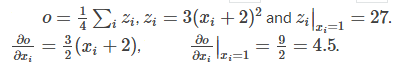
\includegraphics[width=\linewidth,keepaspectratio]{pyt2}
\end{center}
\end{frame}


 %%%%%%%%%%%%%%%%%%%%%%%%%%%%%%%%%%%%%%%%%%%%%%%%%%%%%%%%%%%%%%%%%%%%%%%%%%%%%%%%%%
\begin{frame}[fragile]
\frametitle{Testing}
\begin{itemize}
\item Not creating a graph is extremely useful when we are doing inference, and don't need gradients.
\end{itemize}
   
\end{frame} 

 %%%%%%%%%%%%%%%%%%%%%%%%%%%%%%%%%%%%%%%%%%%%%%%%%%%%%%%%%%%%%%%%%%%%%%%%%%%%%%%%%%
\begin{frame}[fragile]
\frametitle{Testing}
 In Pytorch, you can use LSTM model right away. If we apply iterations, it keeps improving weights, thats it. But you can query prediction at the start itself. That will not be very good as the weights are not stable at that point in time. Prediction needs to be under no\_grad() scope.
 
 \begin{lstlisting}
with torch.no_grad():
    for context, target in test_trigrams:
        context_idxs = torch.tensor([word_to_ix[w] for w in context], dtype=torch.long)
        log_probs = model(context_idxs)
        max_prob_index = np.argmax(log_probs).numpy()
        print(ix_to_word[max_prob_index.item()], " ", target)
\end{lstlisting}     
\end{frame} 

 %%%%%%%%%%%%%%%%%%%%%%%%%%%%%%%%%%%%%%%%%%%%%%%%%%%%%%%%%%%%%%%%%%%%%%%%%%%%%%%%%%
\begin{frame}[fragile]
\frametitle{Example}
 \begin{itemize}
\item Lets write a simple regression workflow using Pytorch syntax but without nn module
\item  
 Inputs are 6 (2d) points and output is corresponding real values, total 6.
 \end{itemize}

 \begin{lstlisting}
from torch.autograd import Variable
import torch

x = Variable(torch.Tensor([[1.0, 1.0], 
                           [1.0, 2.1], 
                           [1.0, 3.6], 
                           [1.0, 4.2], 
                           [1.0, 6.0], 
                           [1.0, 7.0]]))
y = Variable(torch.Tensor([1.0, 2.1, 3.6, 4.2, 6.0, 7.0]))
\end{lstlisting}   

{\tiny (Ref: https://discuss.pytorch.org/t/understanding-how-torch-nn-module-works/122 )} 
\end{frame} 

 %%%%%%%%%%%%%%%%%%%%%%%%%%%%%%%%%%%%%%%%%%%%%%%%%%%%%%%%%%%%%%%%%%%%%%%%%%%%%%%%%%
\begin{frame}[fragile]
\frametitle{Example}
\begin{lstlisting}
weights = Variable(torch.zeros(2, 1), requires_grad=True) # w1, w2

for i in range(5000):
	weight.grad.data.zero_()
    prediction = x.mm(weights) # matrix multiply
    loss = torch.mean((prediction - y)**2)
    loss.backward()
    weights.data.add_(-0.0001 * weights.grad.data) #add_ is inplace
    
    if loss.data[0] < 1e-3:
        break
print('n_iter', i)
print(loss.data[0])
>>>n_iter 1188
0.0004487129335757345
\end{lstlisting}     
\end{frame} 

 %%%%%%%%%%%%%%%%%%%%%%%%%%%%%%%%%%%%%%%%%%%%%%%%%%%%%%%%%%%%%%%%%%%%%%%%%%%%%%%%%%
\begin{frame}[fragile]
\frametitle{Example}
\begin{lstlisting}
import torch.nn.functional as F

class Model(torch.nn.Module):
    
    def __init__(self):
        super(Model, self).__init__()
        #self.weights = Variable(torch.zeros(2, 1), requires_grad=True) # Does not work
		#self.weights = Parameter(torch.zeros(2, 1), requires_grad=True) # Works
		self.fc = torch.nn.Linear(2, 1)
    
    def forward(self, x):
        #prediction = x.mm(self.weights)
        #return prediction
		return self.fc(x) 
        
\end{lstlisting}     
\end{frame} 

 %%%%%%%%%%%%%%%%%%%%%%%%%%%%%%%%%%%%%%%%%%%%%%%%%%%%%%%%%%%%%%%%%%%%%%%%%%%%%%%%%%
\begin{frame}[fragile]
\frametitle{Example}
\begin{lstlisting}
model = Model()
criterion = torch.nn.MSELoss()
optimizer = torch.optim.SGD(model.parameters(), lr=0.001)
loss2 = []

for i in range(5000):
    optimizer.zero_grad()
    outputs = model(x)
    
    loss = criterion(outputs, y)
    loss2.append(loss.data[0])
    loss.backward()        
\end{lstlisting}     
\end{frame} 



%%%%%%%%%%%%%%%%%%%%%%%%%%%%%%%%%%%%%%%%%%%%%%%%%%%
\begin{frame}
  \begin{center}
    {\Large Simple Linear Regression Example}
    
\tiny{(Ref: PyTorchZeroToAll  - Sung Kim)}
  \end{center}
\end{frame}

%%%%%%%%%%%%%%%%%%%%%%%%%%%%%%%%%%%%%%%%%%%%%%%%%%%
\begin{frame}[fragile] \frametitle{Background: Simple Example}
\begin{center}
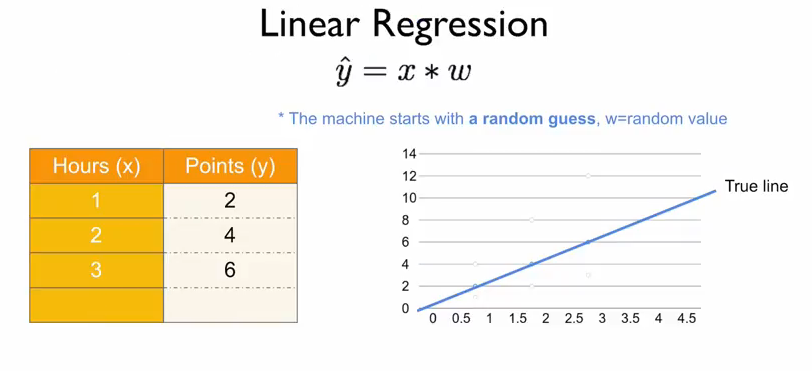
\includegraphics[width=\linewidth,keepaspectratio]{pyhun1}
\end{center}

How solve?


\end{frame}

%%%%%%%%%%%%%%%%%%%%%%%%%%%%%%%%%%%%%%%%%%%%%%%%%%%
\begin{frame}[fragile] \frametitle{Simple Example}
 Start with some $w$, calculate the loss.
\begin{center}
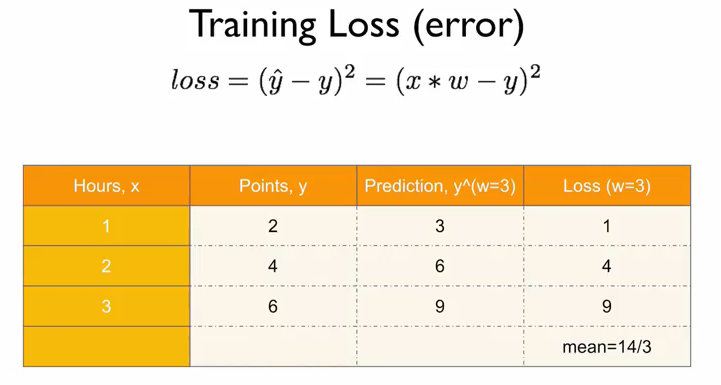
\includegraphics[width=\linewidth,keepaspectratio]{pyhun2}
\end{center}

Plot loss for different $w$ values


\end{frame}


%%%%%%%%%%%%%%%%%%%%%%%%%%%%%%%%%%%%%%%%%%%%%%%%%%%
\begin{frame}[fragile] \frametitle{Simple Example}
 Start with some $w$, calculate the loss.
\begin{center}
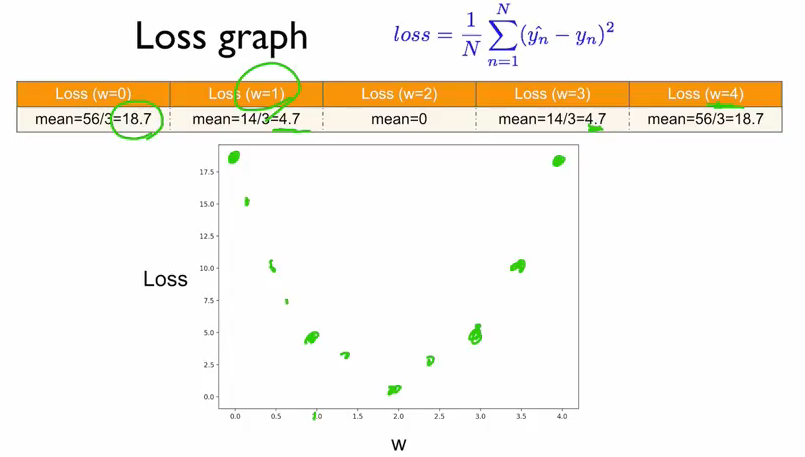
\includegraphics[width=\linewidth,keepaspectratio]{pyhun3}
\end{center}

Plot loss for different $w$ values, and find minimum.

\end{frame}


%%%%%%%%%%%%%%%%%%%%%%%%%%%%%%%%%%%%%%%%%%%%%%%%%%%
\begin{frame}[fragile] \frametitle{Simple Example}
Simple python code looks like:
\begin{center}
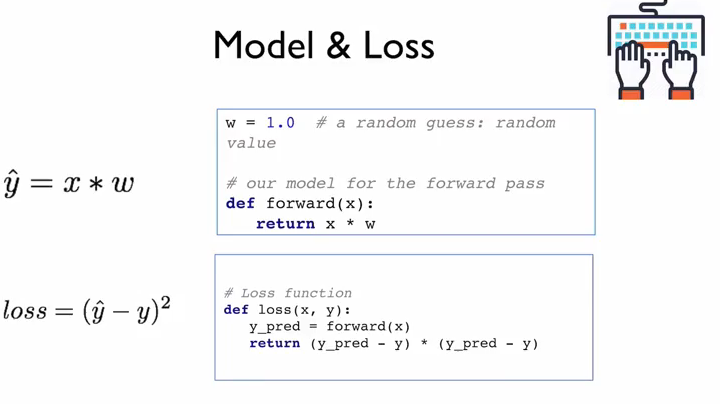
\includegraphics[width=\linewidth,keepaspectratio]{pyhun4}
\end{center}


\end{frame}

%%%%%%%%%%%%%%%%%%%%%%%%%%%%%%%%%%%%%%%%%%%%%%%%%%%
\begin{frame}[fragile] \frametitle{Simple Example}
For data:
\begin{lstlisting}
x_data = [1.0, 2.0, 3.0]
y_data = [2.0, 4.0, 6.0]
\end{lstlisting}

\begin{center}
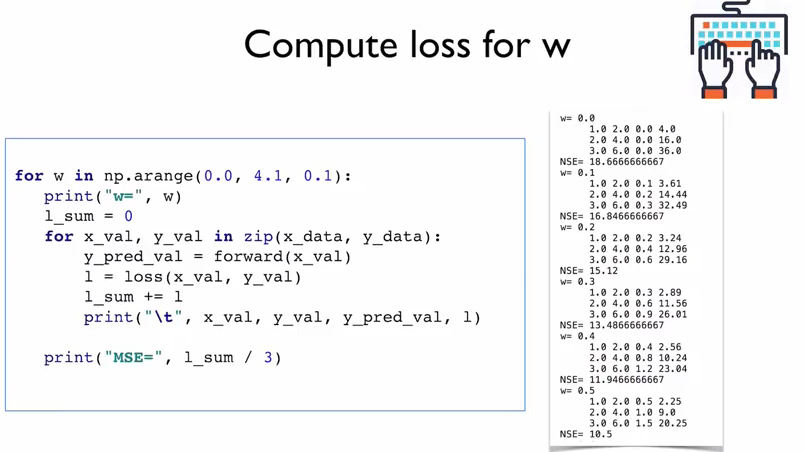
\includegraphics[width=\linewidth,keepaspectratio]{pyhun5}
\end{center}


\end{frame}

%%%%%%%%%%%%%%%%%%%%%%%%%%%%%%%%%%%%%%%%%%%%%%%%%%%
\begin{frame}[fragile] \frametitle{Simple Example}
Entire program:
\begin{center}
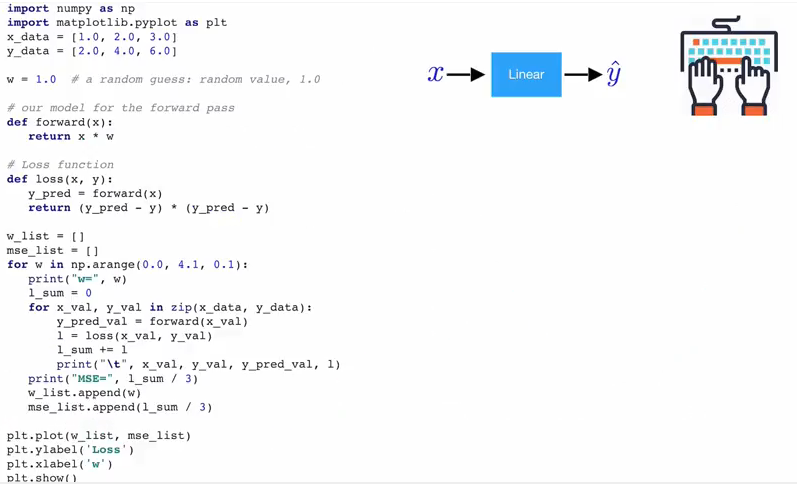
\includegraphics[width=\linewidth,keepaspectratio]{pyhun6}
\end{center}


\end{frame}

%%%%%%%%%%%%%%%%%%%%%%%%%%%%%%%%%%%%%%%%%%%%%%%%%%%
\begin{frame}[fragile] \frametitle{Simple Example}
\begin{center}
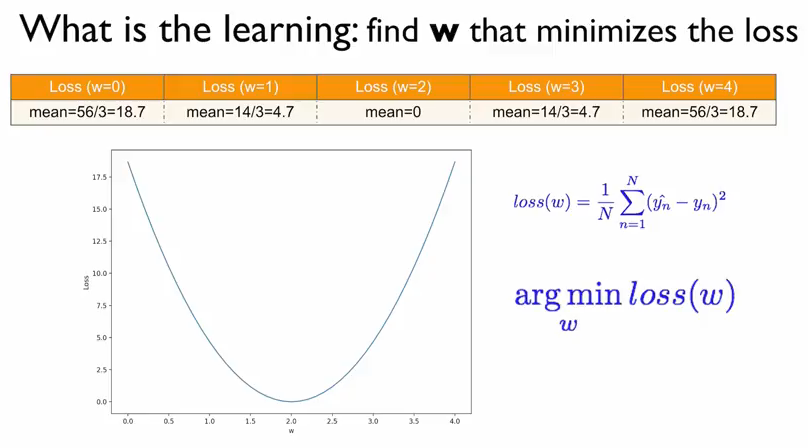
\includegraphics[width=\linewidth,keepaspectratio]{pyhun7}
\end{center}


\end{frame}

%%%%%%%%%%%%%%%%%%%%%%%%%%%%%%%%%%%%%%%%%%%%%%%%%%%
\begin{frame}[fragile] \frametitle{Simple Example}
\begin{center}
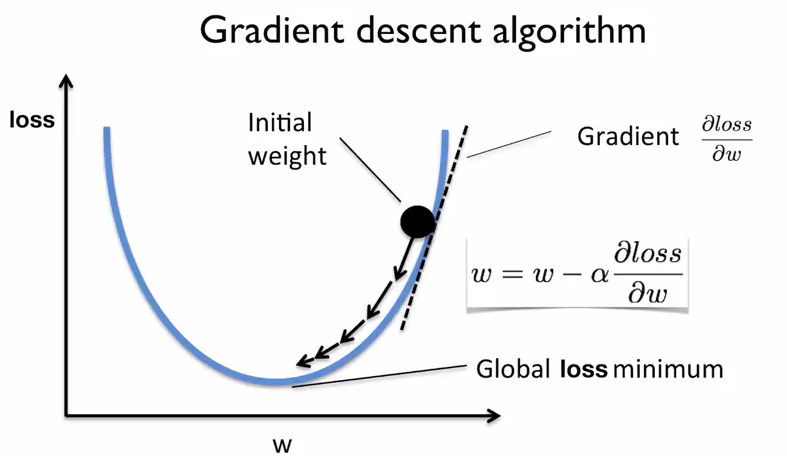
\includegraphics[width=\linewidth,keepaspectratio]{pyhun8}
\end{center}


\end{frame}

%%%%%%%%%%%%%%%%%%%%%%%%%%%%%%%%%%%%%%%%%%%%%%%%%%%
\begin{frame}[fragile] \frametitle{Whats the derivative?}

\begin{center}
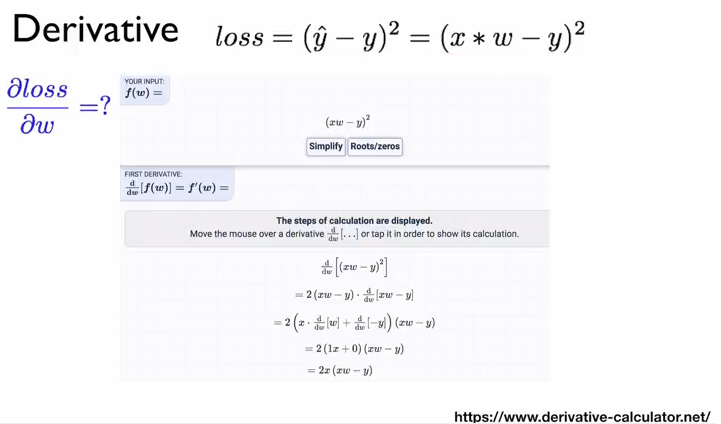
\includegraphics[width=\linewidth,keepaspectratio]{pyhun9}
\end{center}



\end{frame}

%%%%%%%%%%%%%%%%%%%%%%%%%%%%%%%%%%%%%%%%%%%%%%%%%%%
\begin{frame}[fragile] \frametitle{Update}

\begin{center}
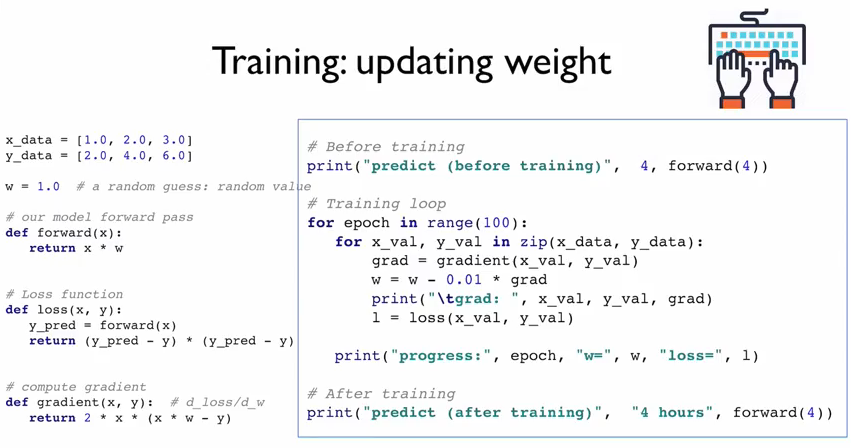
\includegraphics[width=\linewidth,keepaspectratio]{pyhun10}
\end{center}


\end{frame}

%%%%%%%%%%%%%%%%%%%%%%%%%%%%%%%%%%%%%%%%%%%%%%%%%%%
\begin{frame}[fragile] \frametitle{Update}
\begin{itemize}
\item Function for loss seen was simple, we could calculate and implement it easily, but for complicated network, with non-linearity, its not easy.
\item From $x$ to $loss$ there could be many sub-variables in between.
\item Here, we use chain rule. 
\item We calculate gradient at each stage, then the total gradient is just the multiplication of all.
\end{itemize}

\begin{center}
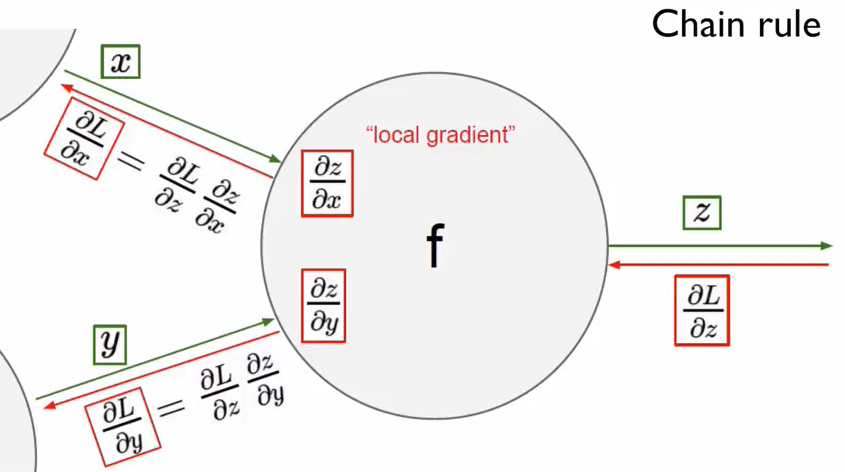
\includegraphics[width=0.5\linewidth,keepaspectratio]{pyhun11}
\end{center}


\end{frame}

%%%%%%%%%%%%%%%%%%%%%%%%%%%%%%%%%%%%%%%%%%%%%%%%%%%
\begin{frame}[fragile] \frametitle{Update}
Example: if $f(x,y) = x.y$ and somehow final gradient is given as 5.
$dz/dx = d(fx,y)/dx = d(x.y)/dx = y$ 

\begin{center}
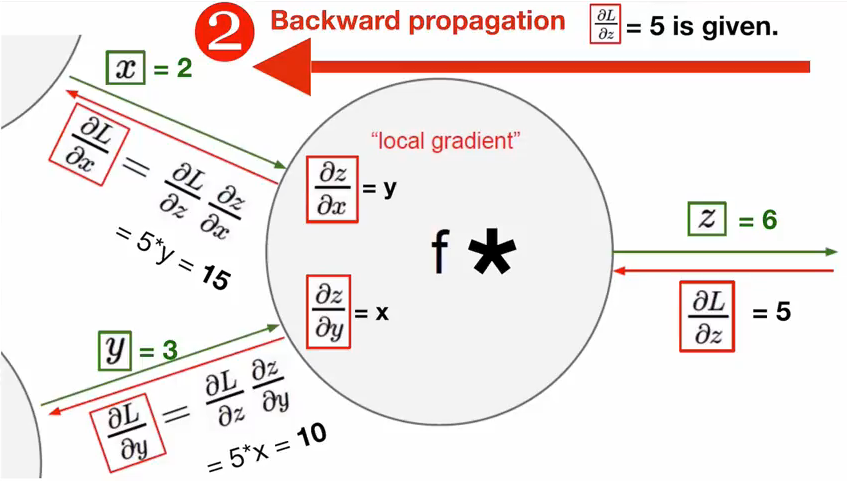
\includegraphics[width=0.8\linewidth,keepaspectratio]{pyhun12}
\end{center}


\end{frame}

%%%%%%%%%%%%%%%%%%%%%%%%%%%%%%%%%%%%%%%%%%%%%%%%%%%
\begin{frame}[fragile] \frametitle{Update}
Computational Graph of the loss function looks like:

\begin{center}
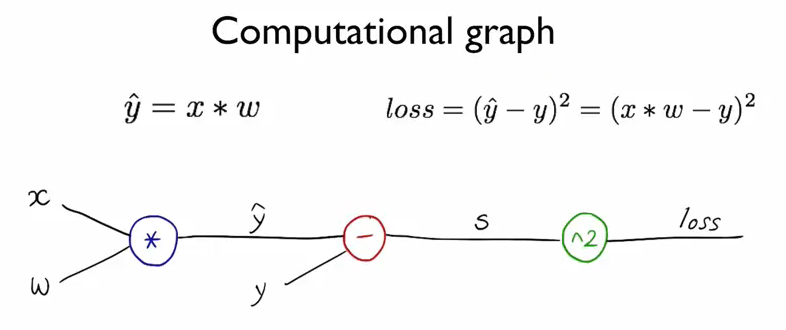
\includegraphics[width=\linewidth,keepaspectratio]{pyhun13}
\end{center}


\end{frame}

%%%%%%%%%%%%%%%%%%%%%%%%%%%%%%%%%%%%%%%%%%%%%%%%%%%
\begin{frame}[fragile] \frametitle{Update}
Forward Pass, with some input and w values:

\begin{center}
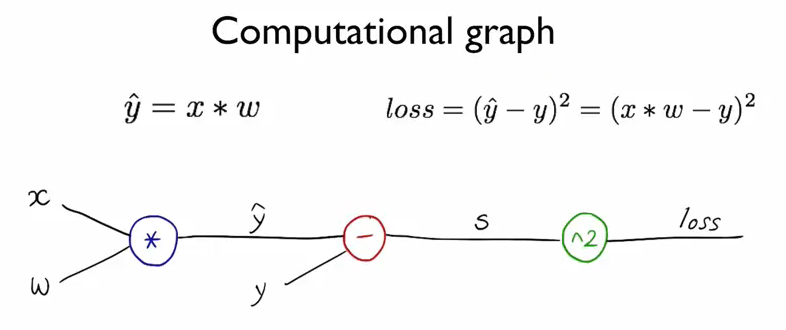
\includegraphics[width=\linewidth,keepaspectratio]{pyhun13}
\end{center}


\end{frame}

%%%%%%%%%%%%%%%%%%%%%%%%%%%%%%%%%%%%%%%%%%%%%%%%%%%
\begin{frame}[fragile] \frametitle{Update}
For backward pass, we need to calculate local gradients. Meaning, around each node.
Say, $s$ is input and $s^2$ is output on the last node. so its derivative is $ds^2/ds$.

\begin{center}
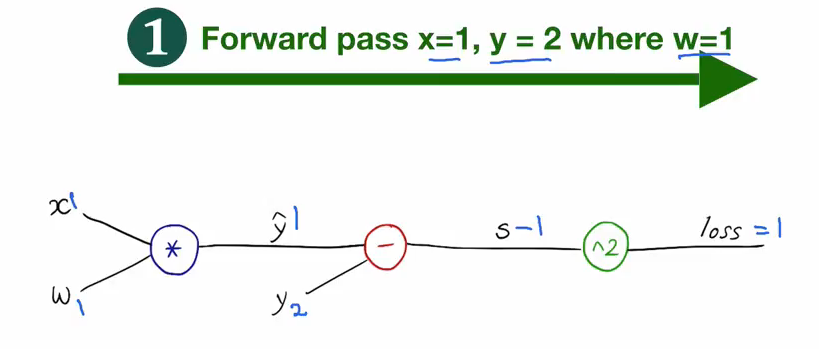
\includegraphics[width=0.8\linewidth,keepaspectratio]{pyhun14}
\end{center}


\end{frame}

%%%%%%%%%%%%%%%%%%%%%%%%%%%%%%%%%%%%%%%%%%%%%%%%%%%
\begin{frame}[fragile] \frametitle{Update}
Total gradient is just multiplication of all the node-wise gradients. Note that gradient is not calculated for x and y as they are input variables.

\begin{center}
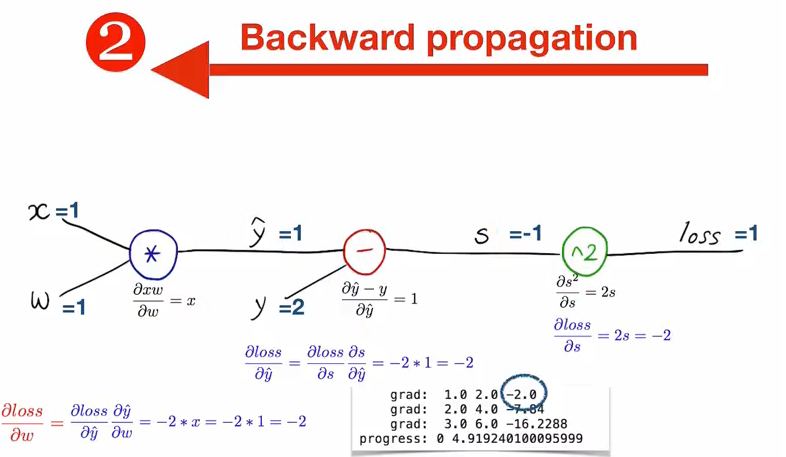
\includegraphics[width=0.7\linewidth,keepaspectratio]{pyhun15}
\end{center}

Final gradient $d(loss)/dw$ is - 2. Update w with it.


\end{frame}


%%%%%%%%%%%%%%%%%%%%%%%%%%%%%%%%%%%%%%%%%%%%%%%%%%%
\begin{frame}[fragile] \frametitle{Update}
No need to compute gradient in pytorch. If you make $w$ as $Variable$ then its calculated automatically, looking at the computation path using it.

\begin{center}
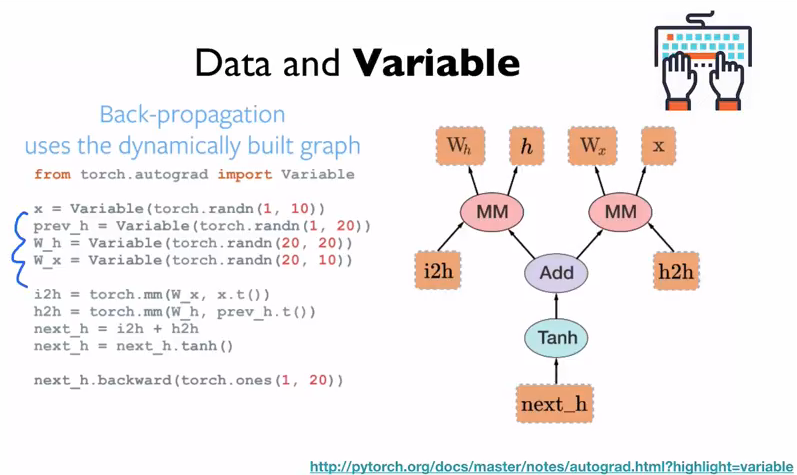
\includegraphics[width=0.7\linewidth,keepaspectratio]{pyhun16}
\end{center}




\end{frame}

%%%%%%%%%%%%%%%%%%%%%%%%%%%%%%%%%%%%%%%%%%%%%%%%%%%
\begin{frame}[fragile] \frametitle{Update}
Pytorch's loss.backward() does back-propagation and the gradient values get stored in w.

\begin{center}
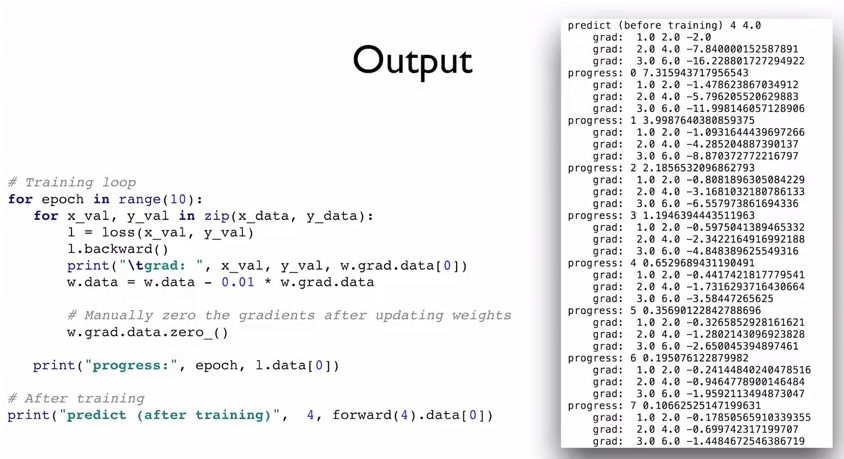
\includegraphics[width=0.8\linewidth,keepaspectratio]{pyhun17}
\end{center}


(Ref: PyTorchZeroToAll  - Sung Kim)
\end{frame}


%%%%%%%%%%%%%%%%%%%%%%%%%%%%%%%%%%%%%%%%%%%%%%%%%%%
\begin{frame}[fragile] \frametitle{Update}
Summary: It calculates all the sub gradients but we are interested in the whole gradient. $w.data$ is w and $w.grad.data$ is the gradient.

\begin{center}
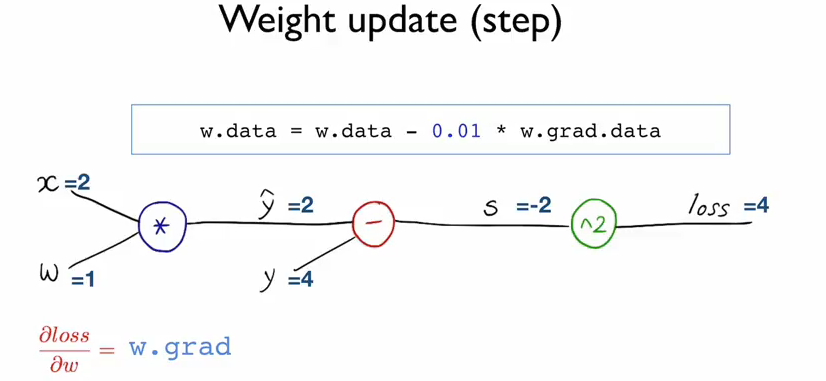
\includegraphics[width=0.8\linewidth,keepaspectratio]{pyhun18}
\end{center}


(Ref: PyTorchZeroToAll  - Sung Kim)
\end{frame}

%%%%%%%%%%%%%%%%%%%%%%%%%%%%%%%%%%%%%%%%%%%%%%%%%%%
\begin{frame}[fragile] \frametitle{Steps in PyTorch}
\begin{itemize}
\item Design Neural Network model inside a class with variables
\item Construct loss and set optimizer
\item Write forward, call backward and put the whole thing in iterations.

\end{itemize}
\end{frame}

%%%%%%%%%%%%%%%%%%%%%%%%%%%%%%%%%%%%%%%%%%%%%%%%%%%
\begin{frame}[fragile] \frametitle{Steps in PyTorch}


\begin{center}
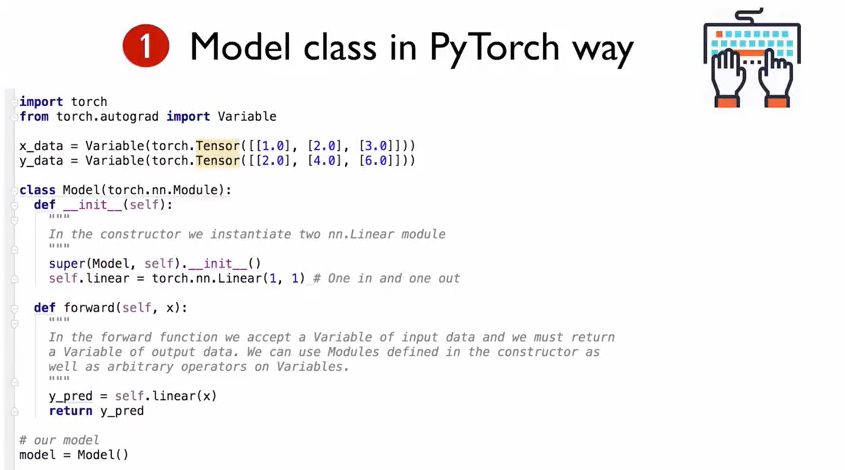
\includegraphics[width=\linewidth,keepaspectratio]{pyhun19}
\end{center}





\end{frame}

%%%%%%%%%%%%%%%%%%%%%%%%%%%%%%%%%%%%%%%%%%%%%%%%%%%
\begin{frame}[fragile] \frametitle{Steps in PyTorch}
\begin{itemize}
\item Inputs and outputs are in the form of tensors (nd-arrays)
\item Your class is derived from nn.Module.
\item Init creates a linear block with 1 input and 1 output.
\item In forward we use the linear block. No external x but its internal to the block.
\item backward() calculates all the gradients in the Variables.
\item step() updates the parameters like, w, which will then be used in the next epoch
\end{itemize}
\end{frame}


%%%%%%%%%%%%%%%%%%%%%%%%%%%%%%%%%%%%%%%%%%%%%%%%%%%
\begin{frame}[fragile] \frametitle{Steps in PyTorch}
In optimizer we do not explicitly ask to minimize w, but it optimizes all (w , b) parameters.

\begin{center}
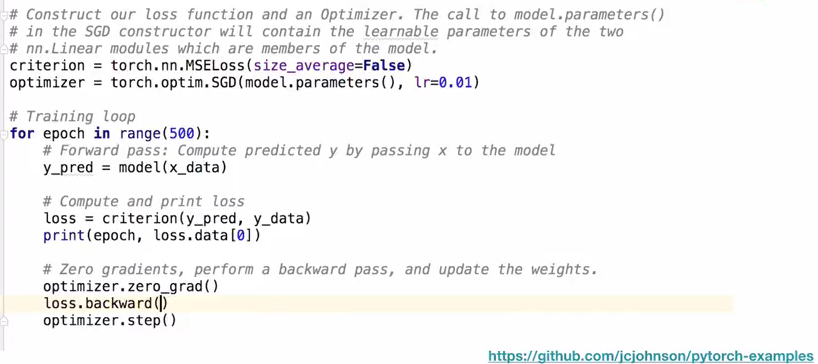
\includegraphics[width=\linewidth,keepaspectratio]{pyhun20}
\end{center}


\end{frame}

%%%%%%%%%%%%%%%%%%%%%%%%%%%%%%%%%%%%%%%%%%%%%%%%%%%
\begin{frame}[fragile] \frametitle{Steps in PyTorch}
Once model is read/stable, we can use to predict.

\begin{center}
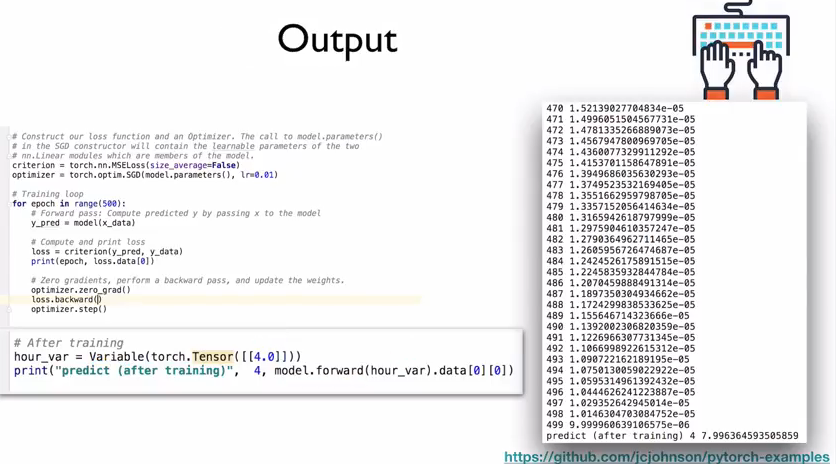
\includegraphics[width=\linewidth,keepaspectratio]{pyhun21}
\end{center}


\end{frame}


%%%%%%%%%%%%%%%%%%%%%%%%%%%%%%%%%%%%%%%%%%%%%%%%%%%
\begin{frame}[fragile] \frametitle{Steps in PyTorch}
To convert linear regression to logistic, just add sigmoid in the forward()

\begin{center}
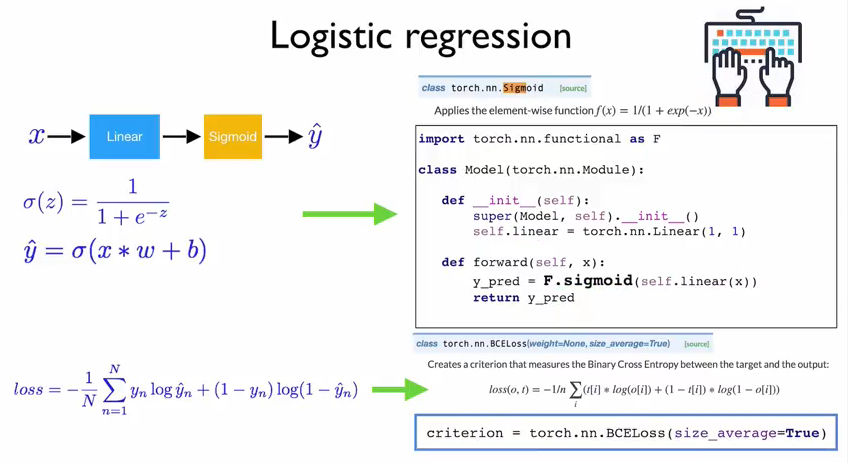
\includegraphics[width=\linewidth,keepaspectratio]{pyhun22}
\end{center}



\end{frame}


%%%%%%%%%%%%%%%%%%%%%%%%%%%%%%%%%%%%%%%%%%%%%%%%%%%
\begin{frame}[fragile] \frametitle{Steps in PyTorch}
Single variable (x) may not have good predictive power. Lets have one more feature, predicting whether the student will get admitted or not.

\begin{center}
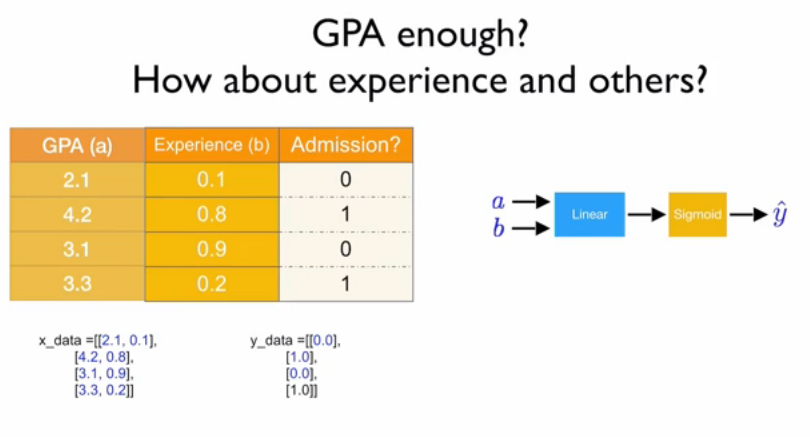
\includegraphics[width=0.8\linewidth,keepaspectratio]{pyhun23}
\end{center}

Use matrix multiplications. Note: Linear model will decide the weights.


\end{frame}

%%%%%%%%%%%%%%%%%%%%%%%%%%%%%%%%%%%%%%%%%%%%%%%%%%%
\begin{frame}[fragile] \frametitle{Steps in PyTorch}
x is matrix. y is also matrix with 1 column. W will thus take such matrix giving $x.w = y$

\begin{center}
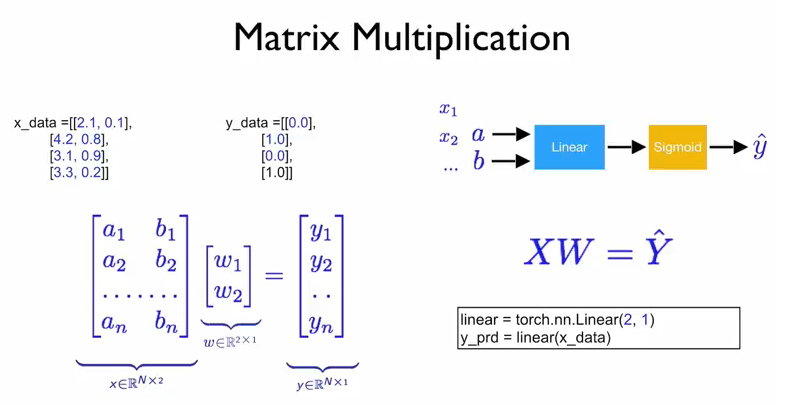
\includegraphics[width=0.8\linewidth,keepaspectratio]{pyhun24}
\end{center}

Use matrix multiplications. Note: Linear model will decide the weights.


\end{frame}


%%%%%%%%%%%%%%%%%%%%%%%%%%%%%%%%%%%%%%%%%%%%%%%%%%%
\begin{frame}[fragile] \frametitle{Steps in PyTorch}
We can have multiple layers. Deep!!

\begin{center}
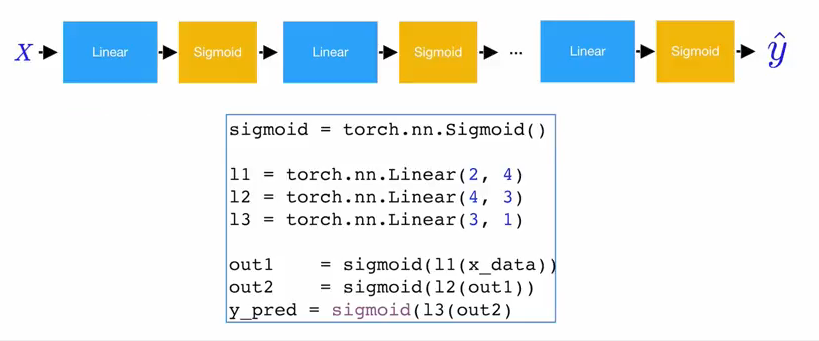
\includegraphics[width=0.8\linewidth,keepaspectratio]{pyhun25}
\end{center}

Make sure you have inputs and ouputs correctly assigned, along with their dimensions.
Inputs and outut dimensions are fixed. Rest you can put anything.
\end{frame}



%%%%%%%%%%%%%%%%%%%%%%%%%%%%%%%%%%%%%%%%%%%%%%%%%%%
\begin{frame}[fragile] \frametitle{Steps in PyTorch}
\begin{itemize}
\item In deep network, Sigmoid can be a problem. 
\item It squashes number to small values (in case of 0/False). 
\item Multiplying such small number, makes gradient vanish in just a few layers.
\item Better to use other activations for internal layers and sigmoid/softmax for the last.
\end{itemize}
\end{frame}


%%%%%%%%%%%%%%%%%%%%%%%%%%%%%%%%%%%%%%%%%%%%%%%%%%%
\begin{frame}[fragile] \frametitle{Example in PyTorch}
\begin{center}
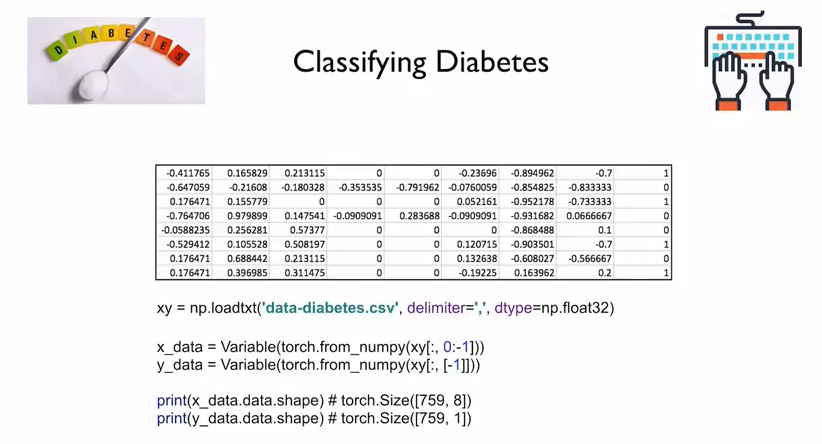
\includegraphics[width=\linewidth,keepaspectratio]{pyhun26}
\end{center}
\end{frame}


%%%%%%%%%%%%%%%%%%%%%%%%%%%%%%%%%%%%%%%%%%%%%%%%%%%
\begin{frame}[fragile] \frametitle{Example in PyTorch}
\begin{center}
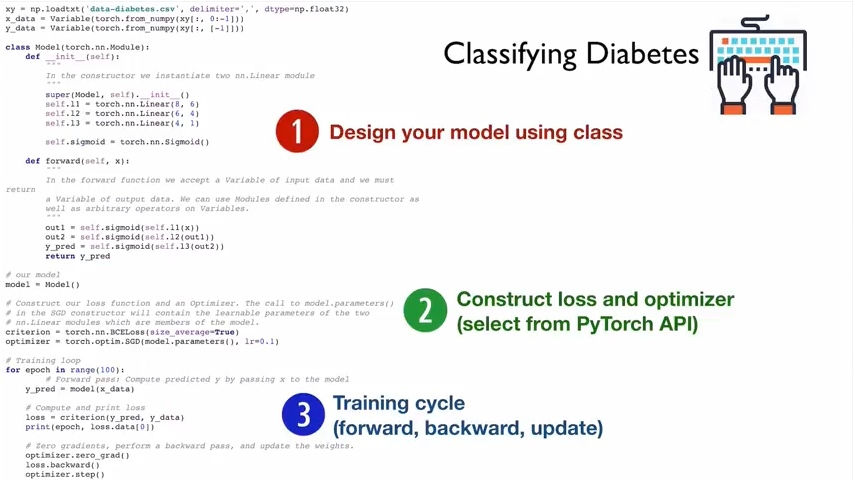
\includegraphics[width=\linewidth,keepaspectratio]{pyhun27}
\end{center}
\end{frame}


%%%%%%%%%%%%%%%%%%%%%%%%%%%%%%%%%%%%%%%%%%%%%%%%%%%
\begin{frame}[fragile] \frametitle{ NN Modules}
\begin{itemize}
\item Modules built on Variable
\item Gradient handled by PyTorch
\item Common Modules
\begin{itemize}
\item  Convolution layers
\item  Linear layers
\item  Pooling layers
\item  Dropout layers
\item  Etc \ldots
\end{itemize}
\end{itemize}
\end{frame}

%%%%%%%%%%%%%%%%%%%%%%%%%%%%%%%%%%%%%%%%%%%%%%%%%%%
\begin{frame}[fragile] \frametitle{Neural Networks}
\begin{itemize}
\item Constructed using the torch.nn package.
\item Contains layers, and a method forward(input)that returns the output.
\end{itemize}
\begin{center}
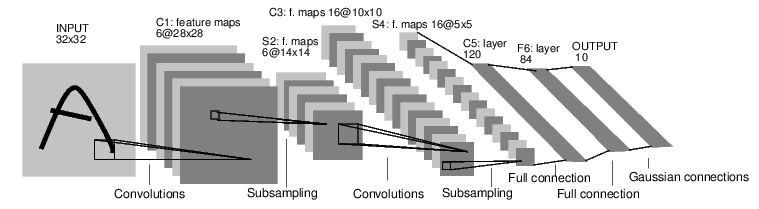
\includegraphics[width=\linewidth,keepaspectratio]{pyt3}
\end{center}
Takes the input, feeds it through several layers one after the other, and then finally gives the output.
\end{frame}

%%%%%%%%%%%%%%%%%%%%%%%%%%%%%%%%%%%%%%%%%%%%%%%%%%%
\begin{frame}[fragile] \frametitle{Convolution Layer}
\begin{itemize}
\item N-th Batch (N), Channel (C)
\item torch.nn.Conv1d: input [N, C, W] \# moving kernel in 1D
\item torch.nn.Conv2d: input [N, C, H, W] \# moving kernel in 2D
\item torch.nn.Conv3d: input [N, C, D, H, W] \# moving kernel in 3D
\item Example: \lstinline|torch.nn.conv2d(in_channels=3, out_channels=16, kernel_size=3, padding=1)|
\end{itemize}
\end{frame}

%%%%%%%%%%%%%%%%%%%%%%%%%%%%%%%%%%%%%%%%%%%%%%%%%%%
\begin{frame}[fragile] \frametitle{Define the network}
\begin{lstlisting}
import torch
from torch.autograd import Variable
import torch.nn as nn
import torch.nn.functional as F

class Net(nn.Module):
	pass
	
net = Net()
print(net)
\end{lstlisting}
\end{frame}

%%%%%%%%%%%%%%%%%%%%%%%%%%%%%%%%%%%%%%%%%%%%%%%%%%%
\begin{frame}[fragile] \frametitle{Define the network}
\begin{lstlisting}
class Net(nn.Module):

    def __init__(self):
        super(Net, self).__init__()
        # 1 input image channel, 6 output channels, 5x5 square convolution
        # kernel
        self.conv1 = nn.Conv2d(1, 6, 5)
        self.conv2 = nn.Conv2d(6, 16, 5)
        # an affine operation: y = Wx + b
        self.fc1 = nn.Linear(16 * 5 * 5, 120)
        self.fc2 = nn.Linear(120, 84)
        self.fc3 = nn.Linear(84, 10)
\end{lstlisting}
\end{frame}



%%%%%%%%%%%%%%%%%%%%%%%%%%%%%%%%%%%%%%%%%%%%%%%%%%%
\begin{frame}[fragile] \frametitle{Define the network}
\begin{lstlisting}
class Net(nn.Module):

    def forward(self, x):
        # Max pooling over a (2, 2) window
        x = F.max_pool2d(F.relu(self.conv1(x)), (2, 2))
        # If the size is a square you can only specify a single number
        x = F.max_pool2d(F.relu(self.conv2(x)), 2)
        x = x.view(-1, self.num_flat_features(x))
        x = F.relu(self.fc1(x))
        x = F.relu(self.fc2(x))
        x = self.fc3(x)
        return x
\end{lstlisting}
\end{frame}

%%%%%%%%%%%%%%%%%%%%%%%%%%%%%%%%%%%%%%%%%%%%%%%%%%%
\begin{frame}[fragile] \frametitle{ Training Procedure}
\begin{itemize}
\item You just have to define the forward function, and the backward function (where gradients are computed) is automatically defined for you using autograd. 
\item You can use any of the Tensor operations in the forward function.
\item The learnable parameters of a model are returned by net.parameters()
\end{itemize}
\begin{lstlisting}
params = list(net.parameters())
print(len(params))
print(params[0].size())  # conv1's .weight

10
torch.Size([6, 1, 5, 5])
\end{lstlisting}

\end{frame}

%%%%%%%%%%%%%%%%%%%%%%%%%%%%%%%%%%%%%%%%%%%%%%%%%%%
\begin{frame}[fragile] \frametitle{ Training Procedure}
\begin{itemize}
\item The input to the forward is an autograd.Variable, and so is the output. 
\item nn.Conv2d will take in a 4D Tensor of nSamples x nChannels x Height x Width 
\item If you have a single sample, just use input.unsqueeze(0) to add a fake batch dimension.
\item Note: Expected input size to this net(LeNet) is 32x32. To use this net on MNIST dataset,please resize the images from the dataset to 32x32
\item Zero the gradient buffers of all parameters and backprops with random gradients:
\end{itemize}
\begin{lstlisting}
net.zero_grad()
out.backward(torch.randn(1, 10))
\end{lstlisting}

\end{frame}


%%%%%%%%%%%%%%%%%%%%%%%%%%%%%%%%%%%%%%%%%%%%%%%%%%%
\begin{frame}[fragile] \frametitle{Define the network}
\begin{lstlisting}
class Net(nn.Module):

    def num_flat_features(self, x):
        size = x.size()[1:]  # all dimensions except the batch dimension
        num_features = 1
        for s in size:
            num_features *= s
        return num_features
\end{lstlisting}
\end{frame}

%%%%%%%%%%%%%%%%%%%%%%%%%%%%%%%%%%%%%%%%%%%%%%%%%%%
\begin{frame}[fragile] \frametitle{Loss Function}
\begin{itemize}
\item A loss function takes the (output, target) pair of inputs, and computes a value that estimates how far away the output is from the target.
\item There are several different loss functions under the nn package . 
\item A simple loss is: nn.MSELoss which computes the mean-squared error between the input and the target.
\end{itemize}
\begin{lstlisting}
output = net(input)
target = Variable(torch.arange(1, 11))  # a dummy target, for example
criterion = nn.MSELoss()

loss = criterion(output, target)
print(loss)

Variable containing:
 38.9008
[torch.FloatTensor of size 1]
\end{lstlisting}

\end{frame}

%%%%%%%%%%%%%%%%%%%%%%%%%%%%%%%%%%%%%%%%%%%%%%%%%%%
\begin{frame}[fragile] \frametitle{Loss Function}
Now, if you follow loss in the backward direction, using it's .grad\_fn attribute, you will see a graph of computations that looks like this:
\begin{lstlisting}
input -> conv2d -> relu -> maxpool2d -> conv2d -> relu -> maxpool2d
      -> view -> linear -> relu -> linear -> relu -> linear
      -> MSELoss
      -> loss
\end{lstlisting}
So, when we call loss.backward(), the whole graph is differentiated w.r.t. the loss, and all Variables in the graph will have their .grad Variable accumulated with the gradient.
\end{frame}

%%%%%%%%%%%%%%%%%%%%%%%%%%%%%%%%%%%%%%%%%%%%%%%%%%%
\begin{frame}[fragile] \frametitle{Loss Function}
For illustration, let us follow a few steps backward:
\begin{lstlisting}
print(loss.grad_fn)  # MSELoss
print(loss.grad_fn.next_functions[0][0])  # Linear
print(loss.grad_fn.next_functions[0][0].next_functions[0][0])  # ReLU

<MseLossBackward object at 0x7ff91efb6ba8>
<AddmmBackward object at 0x7ff91efb6860>
<ExpandBackward object at 0x7ff91efb6860>
\end{lstlisting}

\end{frame}

%%%%%%%%%%%%%%%%%%%%%%%%%%%%%%%%%%%%%%%%%%%%%%%%%%%
\begin{frame}[fragile] \frametitle{Backprop}
\begin{itemize}
\item To backpropagate the error all we have to do is to loss.backward(). 
\item You need to clear the existing gradients though, else gradients will be accumulated to existing gradients
\item Now we shall call loss.backward(), and have a look at conv1's bias gradients before and after the backward.
\end{itemize}
\begin{lstlisting}
net.zero_grad()     # zeroes the gradient buffers of all parameters

print('conv1.bias.grad before backward')
print(net.conv1.bias.grad)

loss.backward()

print('conv1.bias.grad after backward')
print(net.conv1.bias.grad)
\end{lstlisting}

\end{frame}


%%%%%%%%%%%%%%%%%%%%%%%%%%%%%%%%%%%%%%%%%%%%%%%%%%%
\begin{frame}[fragile] \frametitle{Update the weights}
\begin{itemize}
\item $weight = weight - learning_rate * gradient$
\item We can implement this using simple python code:
\end{itemize}
\begin{lstlisting}
learning_rate = 0.01
for f in net.parameters():
    f.data.sub_(f.grad.data * learning_rate)
\end{lstlisting}

\end{frame}


%%%%%%%%%%%%%%%%%%%%%%%%%%%%%%%%%%%%%%%%%%%%%%%%%%%
\begin{frame}[fragile] \frametitle{Update rules}
\begin{itemize}
\item To use various different update rules such as SGD, Nesterov-SGD, Adam, RMSProp, etc. 
\item To enable this, we built a small package: torch.optim that implements all these methods. 
\end{itemize}
\begin{lstlisting}
import torch.optim as optim

# create your optimizer
optimizer = optim.SGD(net.parameters(), lr=0.01)

# in your training loop:
optimizer.zero_grad()   # zero the gradient buffers
output = net(input)
loss = criterion(output, target)
loss.backward()
optimizer.step()    # Does the update
\end{lstlisting}

\end{frame}


%%%%%%%%%%%%%%%%%%%%%%%%%%%%%%%%%%%%%%%%%%%%%%%%%%%
\begin{frame}[fragile] \frametitle{Neural Networks Example}
\begin{center}
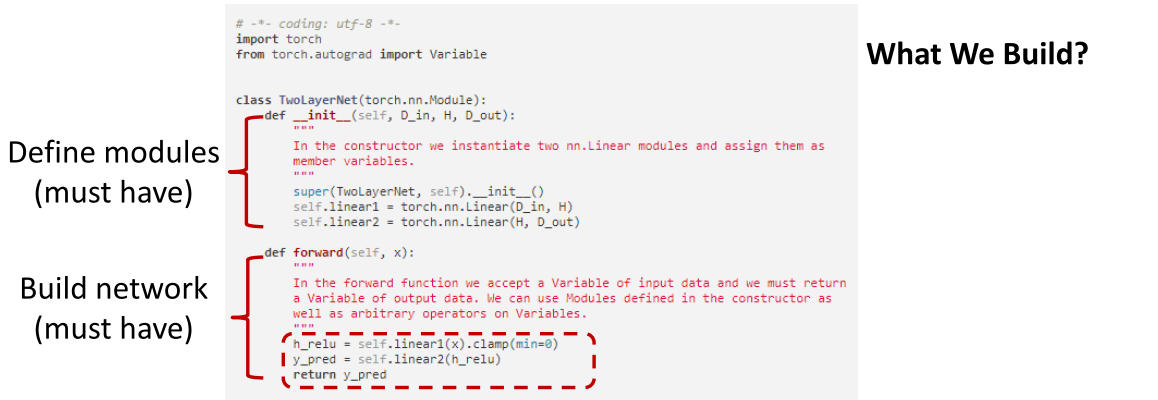
\includegraphics[width=0.8\linewidth,keepaspectratio]{pyt33}
\end{center}
\tiny{(Reference:PyTorch Tutorial-NTU Machine Learning Course-Lyman Lin )}
\end{frame}

%%%%%%%%%%%%%%%%%%%%%%%%%%%%%%%%%%%%%%%%%%%%%%%%%%%
\begin{frame}[fragile] \frametitle{Neural Networks Example}
\begin{center}
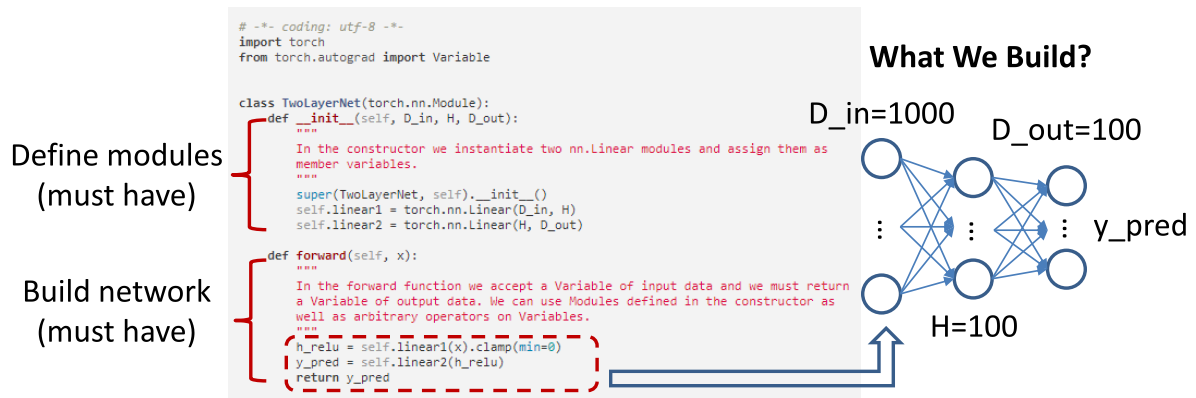
\includegraphics[width=0.8\linewidth,keepaspectratio]{pyt34}
\end{center}
\tiny{(Reference:PyTorch Tutorial-NTU Machine Learning Course-Lyman Lin )}
\end{frame}

%%%%%%%%%%%%%%%%%%%%%%%%%%%%%%%%%%%%%%%%%%%%%%%%%%%
\begin{frame}[fragile] \frametitle{Neural Networks Example}
\begin{center}
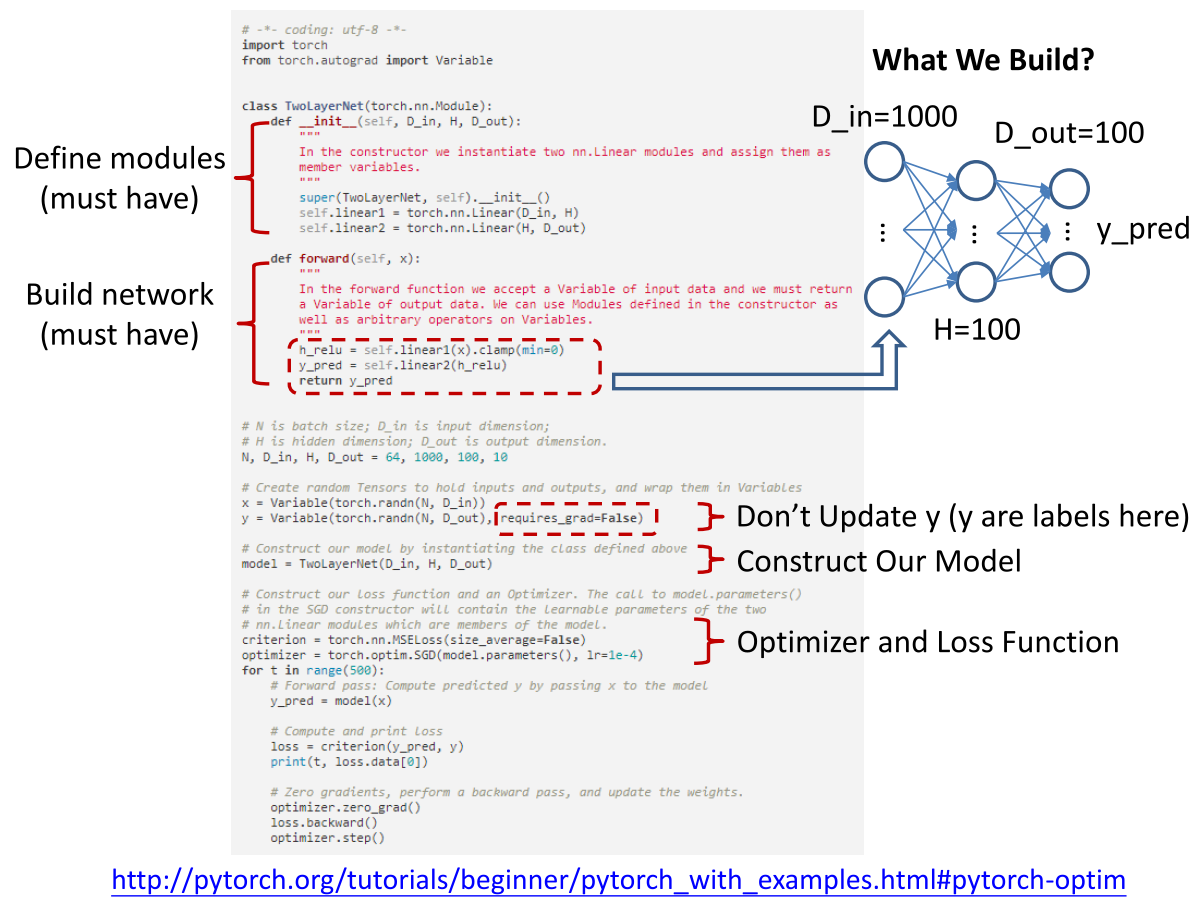
\includegraphics[width=0.8\linewidth,keepaspectratio]{pyt35}
\end{center}
\tiny{(Reference:PyTorch Tutorial-NTU Machine Learning Course-Lyman Lin )}
\end{frame}

%%%%%%%%%%%%%%%%%%%%%%%%%%%%%%%%%%%%%%%%%%%%%%%%%%%
\begin{frame}[fragile] \frametitle{Neural Networks Example}
\begin{center}
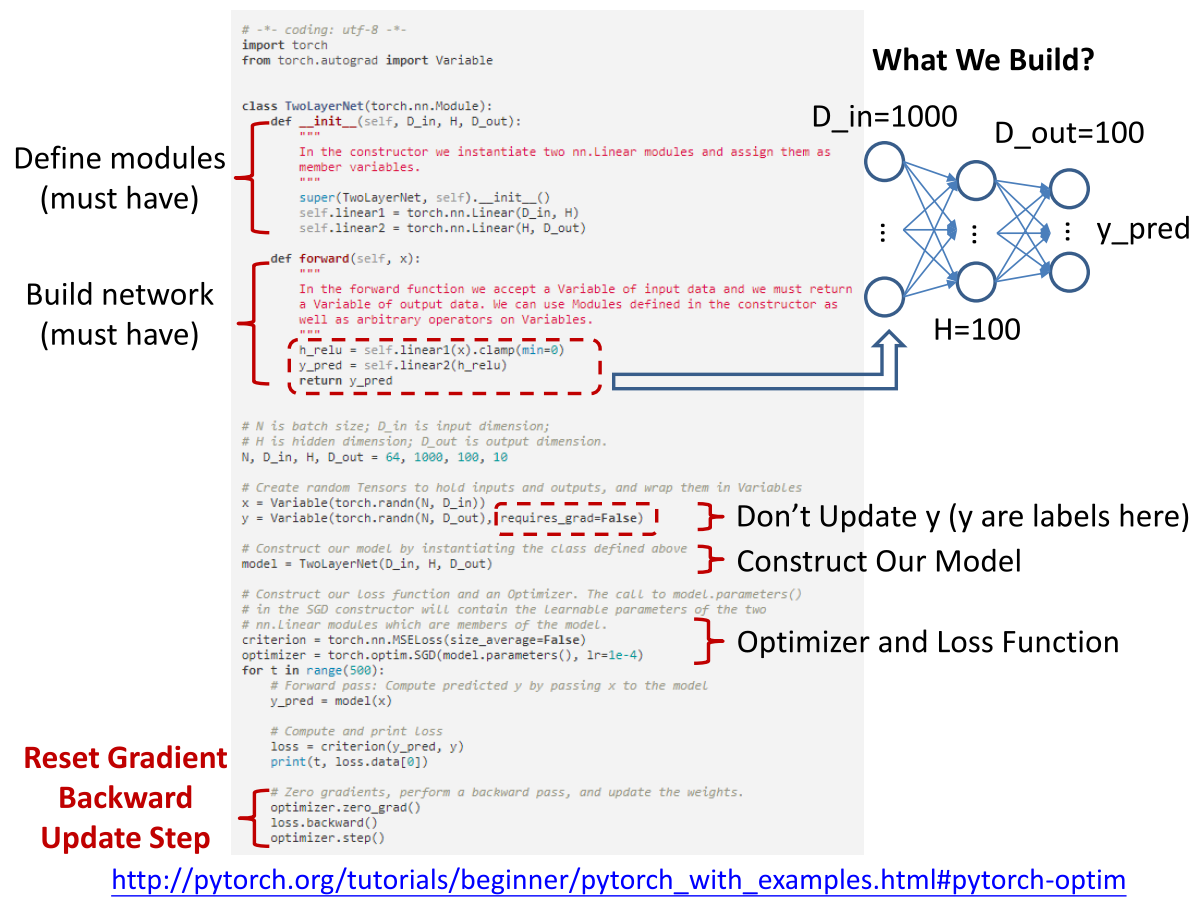
\includegraphics[width=0.8\linewidth,keepaspectratio]{pyt36}
\end{center}
\tiny{(Reference:PyTorch Tutorial-NTU Machine Learning Course-Lyman Lin )}
\end{frame}

%%%%%%%%%%%%%%%%%%%%%%%%%%%%%%%%%%%%%%%%%%%%%%%%%%%
\begin{frame}[fragile] \frametitle{Saving Models}
\begin{itemize}
\item  First Approach (Recommend by PyTorch)
\begin{lstlisting}
# save only the model parameters
torch.save(the_model.state_dict(), PATH)
# load only the model parameters
the_model = TheModelClass(*args, **kwargs)
the_model.load_state_dict(torch.load(PATH))
\end{lstlisting}

\item Second Approach
\begin{lstlisting}
 torch.save(the_model, PATH) # save the entire model
the_model = torch.load(PATH) # load the entire model
\end{lstlisting}
\end{itemize}
\tiny{(Reference:http://pytorch.org/docs/master/notes/serialization.html\#recommended-approach-for-saving-a-model)}
\end{frame}


%%%%%%%%%%%%%%%%%%%%%%%%%%%%%%%%%%%%%%%%%%%%%%%%%%%
\begin{frame}[fragile] \frametitle{Classification Example: MNIST}
Inputs: Images

Output: 10 labels

\begin{center}
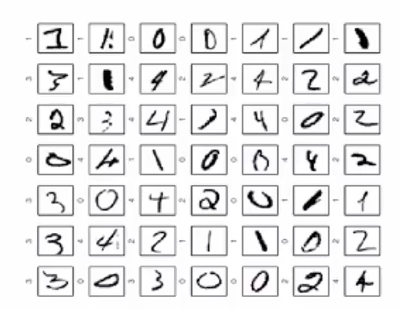
\includegraphics[width=0.6\linewidth,keepaspectratio]{pyhun32}
\end{center}

Logistic regression will give binary output, so sigmoid was ok.

\tiny{(Ref: PyTorchZeroToAll  - Sung Kim)}
\end{frame}

%%%%%%%%%%%%%%%%%%%%%%%%%%%%%%%%%%%%%%%%%%%%%%%%%%%
\begin{frame}[fragile] \frametitle{Classification Example: MNIST}
W matrix size will be mx10. Need softmax activation at the end for multi label classification (probabilities).

\begin{center}
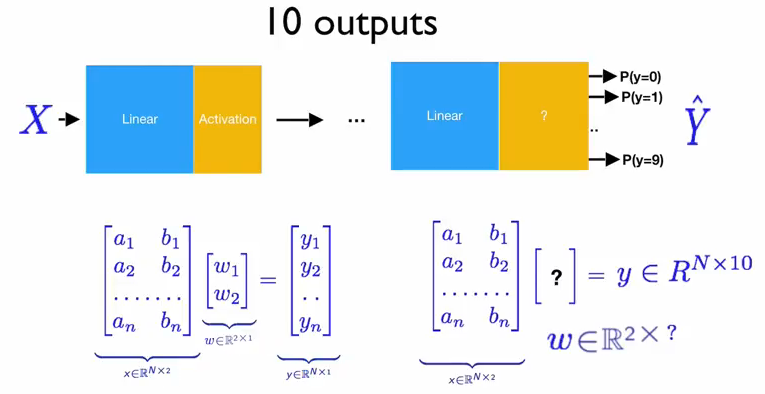
\includegraphics[width=0.8\linewidth,keepaspectratio]{pyhun33}
\end{center}


\tiny{(Ref: PyTorchZeroToAll  - Sung Kim)}
\end{frame}

%%%%%%%%%%%%%%%%%%%%%%%%%%%%%%%%%%%%%%%%%%%%%%%%%%%
\begin{frame}[fragile] \frametitle{Classification Example: MNIST}
Softmax has float input (called logit) and outputs 10 probablilites.

\begin{center}
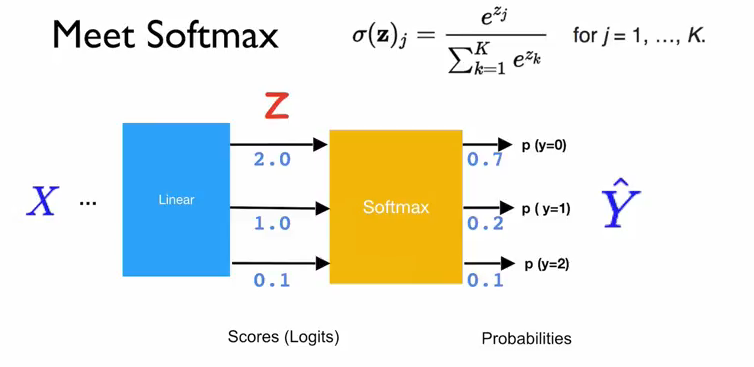
\includegraphics[width=0.8\linewidth,keepaspectratio]{pyhun34}
\end{center}


\tiny{(Ref: PyTorchZeroToAll  - Sung Kim)}
\end{frame}

%%%%%%%%%%%%%%%%%%%%%%%%%%%%%%%%%%%%%%%%%%%%%%%%%%%
\begin{frame}[fragile] \frametitle{Classification Example: MNIST}
Loss is based on cross entropy. Meaning it compares probabilities with one-hot format.

\begin{center}
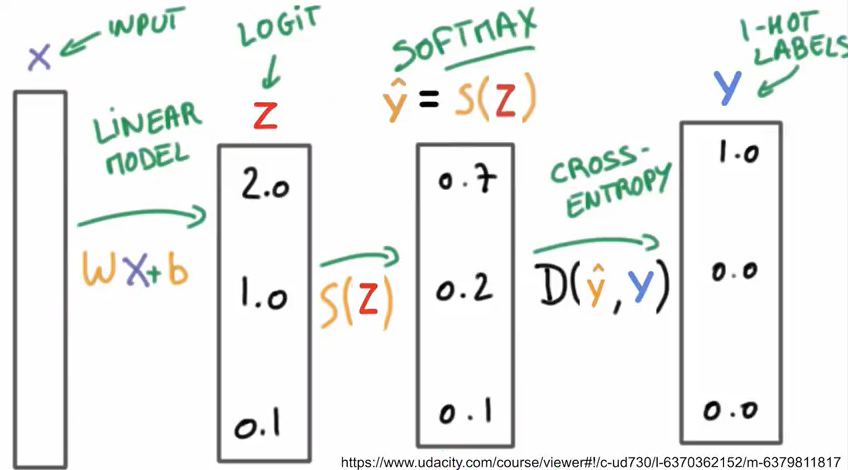
\includegraphics[width=0.8\linewidth,keepaspectratio]{pyhun35}
\end{center}

$D(\hat{Y},Y) = \sum -Y \log \hat{Y}$, where $Y$ and $\hat{Y}$ are two different distributions.

\tiny{(Ref: PyTorchZeroToAll  - Sung Kim)}
\end{frame}

%%%%%%%%%%%%%%%%%%%%%%%%%%%%%%%%%%%%%%%%%%%%%%%%%%%
\begin{frame}[fragile] \frametitle{Classification Example: MNIST}
Pytorch gives a ready loss function. Multiple lables and multiple predictions can also be compared.

\begin{center}
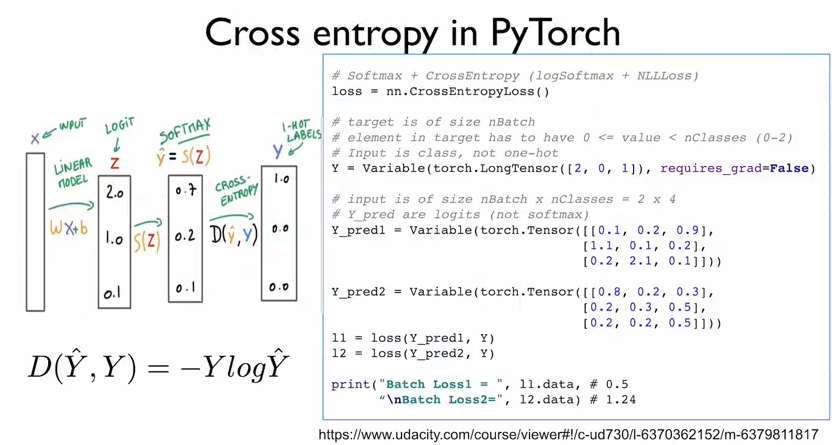
\includegraphics[width=0.8\linewidth,keepaspectratio]{pyhun36}
\end{center}

\tiny{(Ref: PyTorchZeroToAll  - Sung Kim)}
\end{frame}

%%%%%%%%%%%%%%%%%%%%%%%%%%%%%%%%%%%%%%%%%%%%%%%%%%%
\begin{frame}[fragile] \frametitle{Classification Example: MNIST}
\begin{center}
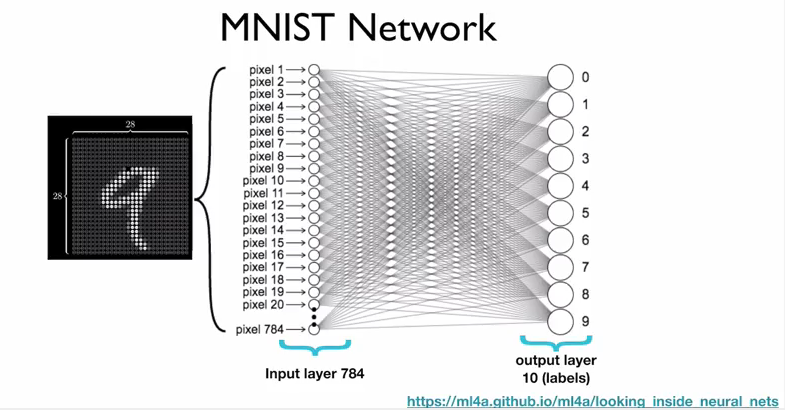
\includegraphics[width=0.8\linewidth,keepaspectratio]{pyhun37}
\end{center}

We can have many hidden layers in between.

\tiny{(Ref: PyTorchZeroToAll  - Sung Kim)}
\end{frame}

%%%%%%%%%%%%%%%%%%%%%%%%%%%%%%%%%%%%%%%%%%%%%%%%%%%
\begin{frame}[fragile] \frametitle{Classification Example: MNIST}
\begin{center}
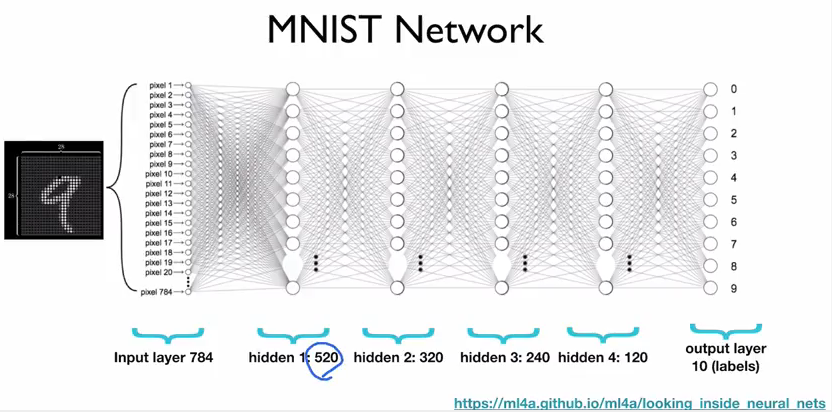
\includegraphics[width=0.8\linewidth,keepaspectratio]{pyhun38}
\end{center}

Weight matrices are set with approprioate dimensions.

\tiny{(Ref: PyTorchZeroToAll  - Sung Kim)}
\end{frame}

%%%%%%%%%%%%%%%%%%%%%%%%%%%%%%%%%%%%%%%%%%%%%%%%%%%
\begin{frame}[fragile] \frametitle{Classification Example: MNIST}
\begin{center}
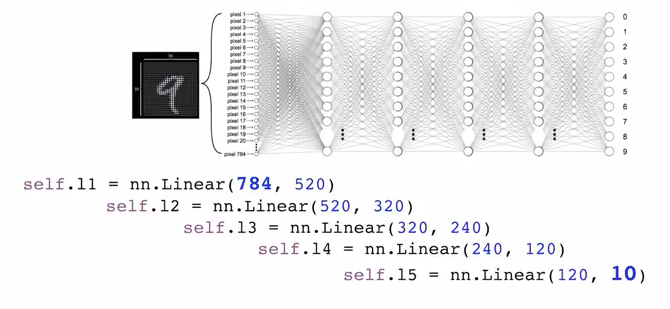
\includegraphics[width=\linewidth,keepaspectratio]{pyhun39}
\end{center}

\tiny{(Ref: PyTorchZeroToAll  - Sung Kim)}
\end{frame}

%%%%%%%%%%%%%%%%%%%%%%%%%%%%%%%%%%%%%%%%%%%%%%%%%%%
\begin{frame}[fragile] \frametitle{Classification Example: MNIST}

Connect the layers in forward() function. We need to reshape it to single vector.

\begin{center}
\includegraphics[width=\linewidth,keepaspectratio]{pyhun40}
\end{center}

\tiny{(Ref: PyTorchZeroToAll  - Sung Kim)}
\end{frame}


%%%%%%%%%%%%%%%%%%%%%%%%%%%%%%%%%%%%%%%%%%%%%%%%%%%
\begin{frame}[fragile] \frametitle{Classification Example: MNIST}

Entire program:

\begin{center}
\includegraphics[width=\linewidth,keepaspectratio]{pyhun41}
\end{center}


\tiny{(Ref: PyTorchZeroToAll  - Sung Kim)}
\end{frame}




%%%%%%%%%%%%%%%%%%%%%%%%%%%%%%%%%%%%%%%%%%%%%%%%%%%
\begin{frame}[fragile] \frametitle{Comparison with TensorFlow}
\begin{center}
\includegraphics[width=0.8\linewidth,keepaspectratio]{pyt37}
\end{center}
\tiny{(Reference:https://awni.github.io/pytorch-tensorflow/ )}
\end{frame}

%%%%%%%%%%%%%%%%%%%%%%%%%%%%%%%%%%%%%%%%%%%%%%%%%%%%%%%%%%%%%%%%%%%%%%%%%%%%%%%%%%
\begin{frame}[fragile]\frametitle{}

\begin{center}
{\Large Deep NLP with Pytorch (0.4.0)}

(Ref: Deep Learning for Natural Language Processing with Pytorch - Robert Guthrie  https://pytorch.org/tutorials/beginner/nlp/pytorch\_tutorial.html)
\end{center}
\end{frame}

 % %%%%%%%%%%%%%%%%%%%%%%%%%%%%%%%%%%%%%%%%%%%%%%%%%%%%%%%%%%%%%%%%%%%%%%%%%%%%%%%%%%
\begin{frame}[fragile]
\frametitle{Pytorch (Recap)}
\begin{itemize}
\item All of deep learning is computations on tensors
\item Array with dimension 0 is a scalar
\item Array with dimension 1 is a vector
\item Array with dimension 2 is a martix
\item Array with dimension 3 or more is a tensor
\item Tensors can be created from Python lists with the torch.Tensor() function.
\end{itemize}
 \end{frame} 
 
 % %%%%%%%%%%%%%%%%%%%%%%%%%%%%%%%%%%%%%%%%%%%%%%%%%%%%%%%%%%%%%%%%%%%%%%%%%%%%%%%%%%
\begin{frame}[fragile]
\frametitle{Pytorch (Recap)}
1D Vector
 \begin{lstlisting}
 import torch
torch.manual_seed(1)

V_data = [1.,2.,3.]
V = torch.Tensor(V_data)
print(V)

>>>tensor([ 1.,  2.,  3.])
 \end{lstlisting}

 \end{frame} 


 
%%%%%%%%%%%%%%%%%%%%%%%%%%%%%%%%%%%%%%%%%%%%%%%%%%%%%%%%%%%%%%%%%%%%%%%%%%%%%%%%%%
\begin{frame}[fragile]
\frametitle{Pytorch (Recap)}
Matrix 
 \begin{lstlisting}
M_data = [[1., 2., 3.], [4., 5., 6]]
M = torch.Tensor(M_data)
print(M)

>>>tensor([[ 1.,  2.,  3.],
        [ 4.,  5.,  6.]])
 \end{lstlisting}

 \end{frame} 

 
 % %%%%%%%%%%%%%%%%%%%%%%%%%%%%%%%%%%%%%%%%%%%%%%%%%%%%%%%%%%%%%%%%%%%%%%%%%%%%%%%%%%
\begin{frame}[fragile]
\frametitle{Pytorch (Recap)}
3D tensor of size 2x2x2.
 \begin{lstlisting}
T_data = [[[1.,2.], [3.,4.]],
          [[5.,6.], [7.,8.]]]
T = torch.Tensor(T_data)
print(T)


>>>tensor([[[ 1.,  2.],
         [ 3.,  4.]],

        [[ 5.,  6.],
         [ 7.,  8.]]])
 \end{lstlisting}

 \end{frame} 

 % %%%%%%%%%%%%%%%%%%%%%%%%%%%%%%%%%%%%%%%%%%%%%%%%%%%%%%%%%%%%%%%%%%%%%%%%%%%%%%%%%%
\begin{frame}[fragile]
\frametitle{Pytorch (Recap)}
\begin{itemize}
\item Indexing into the vector gives you a scalar. 
\item Indexing into the matrix gives you a vector. 
\item Indexing into the tensor gives you a matrix!
\end{itemize}

 \begin{lstlisting}
print(V[0])
print(M[0])
print(T[0])

tensor(1.)
tensor([ 1.,  2.,  3.])
tensor([[ 1.,  2.],
        [ 3.,  4.]])
 \end{lstlisting}

 \end{frame} 
 
 
  % %%%%%%%%%%%%%%%%%%%%%%%%%%%%%%%%%%%%%%%%%%%%%%%%%%%%%%%%%%%%%%%%%%%%%%%%%%%%%%%%%%
\begin{frame}[fragile]
\frametitle{Pytorch (Recap)}
\begin{itemize}
\item Default datatype in tensor is Float
\item For int tensor, call torch.LongTensor(), etc
\item To create a tensor with random data and the supplied dimensionality with torch.randn()
\end{itemize}

 \end{frame} 
 
%%%%%%%%%%%%%%%%%%%%%%%%%%%%%%%%%%%%%%%%%%%%%%%%%%%%%%%%%%%%%%%%%%%%%%%%%%%%%%%%%%
\begin{frame}[fragile]
\frametitle{Pytorch (Recap)}
 \begin{lstlisting}
x = torch.randn((3, 4, 5))
print(x)

>>>tensor([[[-1.5256, -0.7502, -0.6540, -1.6095, -0.1002],
         [-0.6092, -0.9798, -1.6091, -0.7121,  0.3037],
         [-0.7773, -0.2515, -0.2223,  1.6871,  0.2284],
         [ 0.4676, -0.6970, -1.1608,  0.6995,  0.1991]],

        [[ 0.8657,  0.2444, -0.6629,  0.8073,  1.1017],
         [-0.1759, -2.2456, -1.4465,  0.0612, -0.6177],
         [-0.7981, -0.1316,  1.8793, -0.0721,  0.1578],
         [-0.7735,  0.1991,  0.0457,  0.1530, -0.4757]],

        [[-0.1110,  0.2927, -0.1578, -0.0288,  0.4533],
         [ 1.1422,  0.2486, -1.7754, -0.0255, -1.0233],
         [-0.5962, -1.0055,  0.4285,  1.4761, -1.7869],
         [ 1.6103, -0.7040, -0.1853, -0.9962, -0.8313]]])
 \end{lstlisting}

 \end{frame} 
 
 %%%%%%%%%%%%%%%%%%%%%%%%%%%%%%%%%%%%%%%%%%%%%%%%%%%%%%%%%%%%%%%%%%%%%%%%%%%%%%%%%%
\begin{frame}[fragile]
\frametitle{Pytorch (Recap)}
Operations with Tensors
 \begin{lstlisting}
x = torch.Tensor([1.,2.,3.])
y = torch.Tensor([4.,5.,6.])
z = x + y
print(z)

>>>tensor([ 5.,  7.,  9.])
 \end{lstlisting}
Many more mathematical operations are available.
 \end{frame} 
 
%%%%%%%%%%%%%%%%%%%%%%%%%%%%%%%%%%%%%%%%%%%%%%%%%%%%%%%%%%%%%%%%%%%%%%%%%%%%%%%%%%
\begin{frame}[fragile]
\frametitle{Pytorch (Recap)}
Concatenation
 \begin{lstlisting}
# By default, it concatenates along the first axis (concatenates rows)
x_1 = torch.randn(2, 5)
y_1 = torch.randn(3, 5)
z_1 =torch.cat([x_1, y_1])
print(z_1)

# Concatenate columns:
x_2 = torch.randn(2, 3)
y_2 = torch.randn(2, 5)
z_2 = torch.cat([x_2, y_2], 1) # second arg specifies which axis to concat along
print(z_2)

# If your tensors are not compatible, torch will complain.  Uncomment to see the error
# torch.cat([x_1, x_2])
 \end{lstlisting}
 \end{frame} 
 
 %%%%%%%%%%%%%%%%%%%%%%%%%%%%%%%%%%%%%%%%%%%%%%%%%%%%%%%%%%%%%%%%%%%%%%%%%%%%%%%%%%
\begin{frame}[fragile]
\frametitle{Pytorch (Recap)}
Reshaping Tensors with view() method.
 \begin{lstlisting}
x = torch.randn(2,3,4)
print(x)
print(x.view(2,12)) # Reshape to 2 rows, 12 columns
print(x.view(2, -1)) # Same as above. 
 \end{lstlisting}
  If one of the dimensions is -1, its size can be inferred
 \end{frame} 
 
%%%%%%%%%%%%%%%%%%%%%%%%%%%%%%%%%%%%%%%%%%%%%%%%%%%%%%%%%%%%%%%%%%%%%%%%%%%%%%%%%%
\begin{frame}[fragile]
\frametitle{Pytorch (Recap)}
Computation Graphs
\begin{itemize}
\item It is a specification of how your data is combined to give you the output. 
\item Since the graph totally specifies what parameters were involved with which operations, it contains enough information to compute derivatives.
\end{itemize}
 \end{frame} 
 
 
 %%%%%%%%%%%%%%%%%%%%%%%%%%%%%%%%%%%%%%%%%%%%%%%%%%%%%%%%%%%%%%%%%%%%%%%%%%%%%%%%%%
\begin{frame}[fragile]
\frametitle{Pytorch (Recap)}
Variables and Tensors
\begin{itemize}
\item What does torch.Tensor object has stored? : data and the shape, and maybe a few other things
\item But when we added two tensors together, we got an output tensor. 
\item All this output tensor knows is its data and shape. 
\item It has no idea that it was the sum of two other tensors (it could have been read in from a file, it could be the result of some other operation, etc.)
\item The Variable class keeps track of how it was created. 
\end{itemize}
Latest News: Variables and Tensors have merged!!!
 \end{frame} 
 
 
%%%%%%%%%%%%%%%%%%%%%%%%%%%%%%%%%%%%%%%%%%%%%%%%%%%%%%%%%%%%%%%%%%%%%%%%%%%%%%%%%%
\begin{frame}[fragile]
\frametitle{Pytorch (Recap)}
PyTorch 0.4.0 release notes
\begin{itemize}
\item Tensors and Variables have merged
\item torch.autograd.Variable and torch.Tensor are now the same class. 
\item More precisely, torch.Tensor is capable of tracking history and behaves like the old Variable; Variable wrapping continues to work as before but returns an object of type torch.Tensor. \item No need the Variable wrapper everywhere in your code anymore.
\end{itemize}
 \begin{lstlisting}
>>> x = torch.DoubleTensor([1, 1, 1])
>>> print(type(x)) # was torch.DoubleTensor
<class 'torch.autograd.variable.Variable'>
>>> print(x.type())  # OK: 'torch.DoubleTensor'
'torch.DoubleTensor'
>>> print(isinstance(x, torch.DoubleTensor))  # OK: True
True
 \end{lstlisting}
 \end{frame} 
 
    %%%%%%%%%%%%%%%%%%%%%%%%%%%%%%%%%%%%%%%%%%%%%%%%%%%%%%%%%%%%%%%%%%%%%%%%%%%%%%%%%%
\begin{frame}[fragile]
\frametitle{Pytorch (Recap)}
PyTorch 0.4.0 release notes
\begin{itemize}
\item When does autograd start tracking history now?
\item requires\_grad, the central flag for autograd, is now an attribute on Tensors.
\end{itemize}
 \begin{lstlisting}
>>> x = torch.ones(1)  # create a tensor with requires_grad=False (default)
>>> x.requires_grad
False
>>> y = torch.ones(1)  # another tensor with requires_grad=False
>>> z = x + y
>>> # both inputs have requires_grad=False. so does the output
>>> z.requires_grad
False
>>> # then autograd won't track this computation. let's verify!
>>> z.backward()
RuntimeError: element 0 of tensors does not require grad and does not have a grad_fn
 \end{lstlisting}
 \end{frame} 
 
     %%%%%%%%%%%%%%%%%%%%%%%%%%%%%%%%%%%%%%%%%%%%%%%%%%%%%%%%%%%%%%%%%%%%%%%%%%%%%%%%%%
\begin{frame}[fragile]
\frametitle{Pytorch (Recap)}
PyTorch 0.4.0 release notes
 \begin{lstlisting}
>>>
>>> # now create a tensor with requires_grad=True
>>> w = torch.ones(1, requires_grad=True)
>>> w.requires_grad
True
>>> # add to the previous result that has require_grad=False
>>> total = w + z
>>> # the total sum now requires grad!
>>> total.requires_grad
True
>>> # autograd can compute the gradients as well
>>> total.backward()
>>> w.grad
tensor([ 1.])
>>> # and no computation is wasted to compute gradients for x, y and z, which don't require grad
>>> z.grad == x.grad == y.grad == None
True
 \end{lstlisting}
 \end{frame} 
 
     %%%%%%%%%%%%%%%%%%%%%%%%%%%%%%%%%%%%%%%%%%%%%%%%%%%%%%%%%%%%%%%%%%%%%%%%%%%%%%%%%%
\begin{frame}[fragile]
\frametitle{Pytorch (Recap)}
PyTorch 0.4.0 release notes
\begin{itemize}
\item What about .data?
\item .data was the primary way to get the underlying Tensor from a Variable. 
\item After this merge, calling y = x.data still has similar semantics.
\item So y will be a Tensor that shares the same data with x, is unrelated with the computation history of x, and has requires\_grad=False.
\end{itemize}

From now onwards, even if Variables and Tensors are mentioned disticnlty, from 0.4.0, they are just the Tensors with grad\_fn available.
\end{frame} 
 
 
  
  %%%%%%%%%%%%%%%%%%%%%%%%%%%%%%%%%%%%%%%%%%%%%%%%%%%%%%%%%%%%%%%%%%%%%%%%%%%%%%%%%%
\begin{frame}[fragile]
\frametitle{Pytorch (Recap)}
Tensor/Variables operations
 \begin{lstlisting}
x = torch.Tensor([1.,2.,3.])
y = torch.Tensor([4.,5.,6.])
x.requires_grad = True
y.requires_grad = True
z = x + y
print(z.data)
>>>tensor([ 5.,  7.,  9.])
print(z.grad_fn)
>>><AddBackward1 object at 0x000000000A9C94A8>
s = z.sum()
print(s.data)
>>>tensor(21.)
print(s.grad_fn)
>>><SumBackward0 object at 0x000000000A9C94E0>
 \end{lstlisting}
So now, what is the derivative of this sum with respect to the first component of x? 
 \end{frame} 
 
%%%%%%%%%%%%%%%%%%%%%%%%%%%%%%%%%%%%%%%%%%%%%%%%%%%%%%%%%%%%%%%%%%%%%%%%%%%%%%%%%%
\begin{frame}[fragile]
\frametitle{Pytorch (Recap)}
\begin{itemize}
\item Need $\frac{\partial s}{\partial x_0}$
\item s knows that it was created as a sum of the tensor z. 
\item z knows that it was the sum x + y. 
\item So, $s = \overbrace{x_0 + y_0}^\text{$z_0$} + \overbrace{x_1 + y_1}^\text{$z_1$} + \overbrace{x_2 + y_2}^\text{$z_2$}$
\item Enough information to determine that the derivative : Pytorch knows how to compute their gradients of sum() and + operations, and run the back propagation algorithm. 
\end{itemize}


\end{frame} 
 
 %%%%%%%%%%%%%%%%%%%%%%%%%%%%%%%%%%%%%%%%%%%%%%%%%%%%%%%%%%%%%%%%%%%%%%%%%%%%%%%%%%
\begin{frame}[fragile]
\frametitle{Pytorch (Recap)}

 \begin{lstlisting}
s.backward() # calling .backward() on any variable will run backprop, starting from it.
print(x.grad)

>>>tensor([ 1.,  1.,  1.])
 \end{lstlisting}

\end{frame} 
 
 
  %%%%%%%%%%%%%%%%%%%%%%%%%%%%%%%%%%%%%%%%%%%%%%%%%%%%%%%%%%%%%%%%%%%%%%%%%%%%%%%%%%
\begin{frame}[fragile]
\frametitle{Pytorch (Recap)}
Note:
 \begin{lstlisting}
x = torch.randn((2,2))
y = torch.randn((2,2))
x.requires_grad = True
y.requires_grad = True
z = x + y 
print(z.grad_fn)
>>><AddBackward1 object at 0x000000000A9D2358>

var_z_data = z.data # Get the wrapped Tensor object out of var_z...
new_var_z = torch.Tensor( var_z_data ) # Re-wrap the tensor in a new variable

# does new_var_z have info to backprop to x and y? NO!
print(new_var_z.grad_fn)
>>>None
# And how could it?  We copied the tensor values out of z (that is what z.data is).  This tensor doesn't know anything about how it was computed.   If var_z_data doesn't know how it was computed, theres no way new_var_z will.
\end{lstlisting}

\end{frame} 
 
 
%%%%%%%%%%%%%%%%%%%%%%%%%%%%%%%%%%%%%%%%%%%%%%%%%%%%%%%%%%%%%%%%%%%%%%%%%%%%%%%%%%
\begin{frame}[fragile]
\frametitle{Pytorch (Recap)}

\begin{itemize}
\item Neural network consists of composing linearities with non-linearities, a long chains of affine compositions.
\item Non-linearities like $\tanh(x), \sigma(x), \text{ReLU}(x)$ are the most common.
\item Why these functions? I can think of plenty of other non-linearities.
\end{itemize}
\end{frame} 

%%%%%%%%%%%%%%%%%%%%%%%%%%%%%%%%%%%%%%%%%%%%%%%%%%%%%%%%%%%%%%%%%%%%%%%%%%%%%%%%%%
\begin{frame}[fragile]
\frametitle{Pytorch (Recap)}
Activation
\begin{itemize}
\item The reason for this is that they have gradients that are easy to compute, and computing gradients is essential for learning. For example $ \frac{d\sigma}{dx} = \sigma(x)(1 - \sigma(x)) $
\item $ \sigma(x)$ less popular because the gradient vanishes very quickly as the absolute value of the argument grows. Small gradients means it is hard to learn. Most use tanh or ReLU.
\end{itemize}
 \begin{lstlisting}
data = torch.randn(2,2,requires_grad=True)
print(data)
import torch.nn.functional as F
print(F.relu(data))
>>>tensor([[ 1.6169, -0.9026],
        [ 0.1737,  0.0772]])
tensor([[ 1.6169,  0.0000],
        [ 0.1737,  0.0772]])
 \end{lstlisting}
 Note, all negatives are made 0 and positives kept as they are.
\end{frame} 

%%%%%%%%%%%%%%%%%%%%%%%%%%%%%%%%%%%%%%%%%%%%%%%%%%%%%%%%%%%%%%%%%%%%%%%%%%%%%%%%%%
\begin{frame}[fragile]
\frametitle{Pytorch (Recap)}
Softmax and Probabilities
\begin{itemize}
\item The function $\text{Softmax}(x)$ is also just a non-linearity, but it is special in that it usually is the last operation done in a network. 
\item This is because it takes in a vector of real numbers and returns a probability distribution.
\end{itemize}
 \begin{lstlisting}
data = torch.randn(5,requires_grad=True)
print(data)
print(F.softmax(data,0))
print(F.softmax(data,0).sum())

>>>tensor([ 0.1896, -0.2204,  0.1491,  0.0100, -0.1243])
tensor([ 0.2387,  0.1584,  0.2292,  0.1994,  0.1744])
tensor(1.)
 \end{lstlisting}
It should be clear that the output is a probability distribution: each element is non-negative and the sum over all components is 1.
\end{frame} 

%%%%%%%%%%%%%%%%%%%%%%%%%%%%%%%%%%%%%%%%%%%%%%%%%%%%%%%%%%%%%%%%%%%%%%%%%%%%%%%%%%
\begin{frame}[fragile]
\frametitle{Pytorch (Recap)}
Objective or Loss or Cost function
\begin{itemize}
\item Neural network is being trained to minimize it.
\item The parameters of the model are then updated by taking the derivative of the loss function. 
\item An example loss function is the negative log likelihood loss, which is a very common objective for multi-class classification.
\item We can compute gradients with respect to all of the parameters used to compute it! Then we can perform standard gradient updates.
\item Let $\theta$ be our parameters,  $L(\theta)$ the loss function, and $\eta$ a positive learning rate. Then:

$$ \theta^{(t+1)} = \theta^{(t)} - \eta \nabla_\theta L(\theta) $$
\end{itemize}

\end{frame} 

%%%%%%%%%%%%%%%%%%%%%%%%%%%%%%%%%%%%%%%%%%%%%%%%%%%%%%%%%%%%%%%%%%%%%%%%%%%%%%%%%%
\begin{frame}[fragile]
\frametitle{Pytorch (Recap)}
Optimization
\begin{itemize}
\item Many optimization methods do something more than just this vanilla gradient update.
\item Many attempt to vary the learning rate based on what is happening at train time. 
\item Torch provies many in the torch.optim package, and they are all completely transparent. 
\item Using the simplest gradient update is the same as the more complicated algorithms. 
\item Trying different algorithms and different parameters 
\item Other choices: Adam or RMSProp will boost performance noticably.
\end{itemize}

\end{frame} 

%%%%%%%%%%%%%%%%%%%%%%%%%%%%%%%%%%%%%%%%%%%%%%%%%%%%%%%%%%%%%%%%%%%%%%%%%%%%%%%%%%
\begin{frame}[fragile]
\frametitle{Pytorch (Recap)}
Neural Network Architecture
\begin{itemize}
\item Should inherit from nn.Module and override the forward() method.
\item  nn.Module makes it keep track of its trainable parameters, you can swap it between CPU and GPU with the .cuda() or .cpu() functions, etc.
\end{itemize}

\end{frame} 
